% Monografia para Projeto de Fim de Curso - Exemplo no LaTeX
%-----------------------------------------------------------


%---------------Inicialização de pacotes--------------------

\documentclass[12pt,a4paper,notitlepage,twoside]{book}

\usepackage{graphicx}
\usepackage[utf8]{inputenc}
\usepackage[brazil]{babel}		
\usepackage[T1]{fontenc}
\usepackage{amsmath,amssymb}
\usepackage{amsthm,amsfonts}
\usepackage[short]{optidef}
\usepackage{color}
\usepackage[hidelinks]{hyperref}

\usepackage{abntex2abrev}
\usepackage[num, overcite, abnt-emphasize=bf, abnt-etal-list=3]{abntex2cite} 
\citebrackets()

\usepackage{setspace}
\usepackage{parskip}
\usepackage[toc,page]{appendix}
\usepackage[framed, numbered]{matlab-prettifier}

\usepackage{import}
\usepackage{tikz}
\usepackage{booktabs}
\usepackage{float}
\usepackage[skip=10pt]{caption}

\usepackage[a4paper,top=30mm,bottom=30mm,inner=30mm,outer=25mm,headheight=7mm,headsep=6mm,footskip=7mm]{geometry}
\usepackage{enumerate}

\usepackage{svg}

\makeindex

\setstretch{1.03} %%um pouco melhor que espaçamento simples

%---------------Início do documento-------------------------

\begin{document}

\begin{titlepage}
\begin{center}
{\large Universidade Federal de Minas Gerais\\
Escola de Engenharia \\
Curso de Graduação em Engenharia de Controle e Automação\\}

\vspace{6cm}
{\bf\Large Primeira Linha do Título\vspace{0.2cm}

Segunda Linha do Título, se Houver}
\vspace{4cm}

%\hspace{0.3\textwidth} \parbox{0.65\textwidth}
{\large Fulano de Tal}
\vspace{2cm}  
   
\vspace{2cm}          
%\hspace{0.3\textwidth} 
{\large Orientador: Prof. Beltrano, Dr.}\\
{\large Supervisor: Eng. Cicrano}

\vfill
%\hspace{0.3\textwidth} 
{\large Belo Horizonte, Julho de 2014 }
\end{center}

\end{titlepage}

\newpage
\clearpage
\thispagestyle{empty}


\begin{titlepage}

\centering
\textbf{Monografia}\\
\vspace{2cm}
\centering
\textbf{Título da Monografia}\\
\vspace{5cm} 

\parbox{1.0\textwidth} 
{\large 
Monografia submetida à banca examinadora
designada pelo Colegiado Didático do Curso de
Graduação em Engenharia de Controle e
Automação da Universidade Federal de Minas
Gerais, como parte dos requisitos para aprovação na
disciplina Projeto Final de Curso II.}

\vspace{7cm} 
\centering
Belo Horizonte, Julho de 2014

\end{titlepage}


\pagenumbering{roman}
\addcontentsline{toc}{chapter}{Resumo}

\begin{center}
\huge{{\bf Resumo}}
\vspace{2cm}
\end{center}

% No Resumo, em uma única página, em no máximo dois parágrafos, você explicita os seguintes itens: objetivos do projeto e descrição sucinta do local onde ele foi desenvolvido; metodologia utilizada; e resultados alcançados. Leitores experientes decidem se prosseguirão para a leitura do texto completo após lerem o resumo, a conclusão e a introdução. Por isso nestes lugares você deve colocar um esforço maior de convencimento. Além disso, a linguagem utilizada deve ser acessível a leitores com pouca familiaridade com a área, limitando o uso de jargões.
 
% \begin{sloppypar}
% Este novo parágrafo serve para mostrar que ao pular uma ou mais linhas no texto do arquivo .tex, o \TeX\ entende que você está iniciando outro parágrafo. O comando sloppypar força o texto a não ultrapassar as margens. Só deve ser usado se este problema ocorrer.
% \end{sloppypar}

O veículo elétrico da UFMG, o DT1, é um protótipo utilizado em competições de eficiência energética.
A atual medição de seu consumo é de $226,9$~[km/kWh] realizada na competição estudantil Shell EcoMarathon Americas de 2019.
Este projeto de fim de curso tem como objetivo determinar, a partir da aplicação da teoria de controle ótimo, o sinal de controle em malha aberta para acionamento do motor 
elétrico (estrátegia de pista) e a relação de transmissão para que o consumo do DT1 seja o minimo possível na atual pista da competição Shell EcoMarathon Americas no kartódromo de Sonoma.

Para realizar este objetivo, primeiramente foi determinado um modelo matemático da dinâmica longitudinal do veículo protótipo. Com base neste modelo
e nas determinações da organização Shell EcoMarathon para a medição da autonomia foi formulado um problema de controle ótimo que foi resolvido utilizando o
\textit{software} FALCON.m. 

A estrategia de pista e a relação de transmissão encontradas levariam o consumo do protótipo para $905,7$~[km/kWh]. Uma vez que o modelo do protótipo 
não foi validado experimentalmente não foi possível afirmar que está estrategia e esta relação de transmissão são ótimas para o caso real. Contudo foi possível
obter as seguintes conclusões: o motor deve ser ligado no trechos de maior aclive da pista e o tempo total gasto deve ser o máximo permitido. 
 
\textbf{Palavras-chave} -- Veículo Elétrico, Eficiência Energética, Competição Shell EcoMarathon, Modelo Veícular, Problema de Controle Ótimo, FALCON.m.

\clearpage
\thispagestyle{empty}
\cleardoublepage


\addcontentsline{toc}{chapter}{Abstract}

\begin{center}
\huge{{\bf Abstract}}
\vspace{2cm}
\end{center}

The UFMG's electric vehicle, the DT1, is a prototype used in energy efficiency competitions.
The current measurement of your consumption is $226.9$~[km/kWh] performed at the 2019 Shell EcoMarathon Americas student competition.
This end-of-course project aims to determine, based on the application of the optimal control theory, the open loop control signal for motor activation
electric (track strategy) and the transmission ratio so that the consumption of the DT1 is as little as possible on the current track of the Shell EcoMarathon Americas competition at the Sonoma kart track.

To achieve this goal, a mathematical model of the longitudinal dynamics of the prototype vehicle was first determined. Based on this model
and in the determinations of the Shell EcoMarathon organization for an autonomy duration, an optimal control problem was formulated that was solved using the
\textit{software} FALCON.m.

The track strategy and gear ratio found would take the prototype's consumption to $905.7$~[km/kWh]. The prototype model
it was not validated experimentally it was not possible to state that this strategy and this transmission ratio are great for the real case. However it was possible
obtain the following rights: the engine must be started in the most active sections of the track and the total time spent must be the maximum allowed.

\textbf{Keywords} -- Electric Vehicle, Energy Efficiency, Shell EcoMarathon Competition, Vehicle Model, Optimal Control Problem, FALCON.m.

 
\clearpage
\thispagestyle{empty}
\cleardoublepage


\addcontentsline{toc}{chapter}{Agradecimentos}

\begin{center}
\huge{{\bf Agradecimentos}}
\vspace{4cm}
\end{center}

Aos meus pais Vera e Rodeney, à minha irmã Jéssika e à minha noiva Rafaela pelo incentivo e amor. Aos professores Dimas Dutra, Victor Campos e Fabrício Pujatti pelo
apoio, orientação e transferência de conhecimento. Aos membros da equipe de competição Milhagem UFMG pela amizade e pela oportunidade de trabalhar com vocês. À todos que direta
ou indiretamente fizeram parte da minha trajetória, a minha sincera gratidão.
 
\clearpage
\thispagestyle{empty}
\cleardoublepage
\include{TabelaConteudo/TabelaConteudo}
\include{ListaFiguras/ListaFiguras}
\include{ListaTabelas/ListaTabelas}

\pagenumbering{arabic}
\setcounter{page}{1}
\chapter{Introdução}
\label{chap:intro}
\thispagestyle{empty}

Este capítulo explica a motivação e objetivos deste projeto de otimização do desempenho em competições de um veículo elétrico protótipo de alta eficiência.
Apresenta a equipe de competição estudantil Milhagem UFMG onde este PFC foi realizado. E, também, descreve a estrutura desta monografia.

\section{Motivação e Justificativa}
\label{sec:motivacao}

A equipe Milhagem UFMG constrói protótipos de veículos para participar de competições
de eficiência energética. Atualmente a equipe possui dois veículos: o M84 equipado com um motor a combustão interna a gasolina e o DT1,
 apresentado na Figura \ref{fig:DT1}, que possui motor elétrico e bateria. As competições em que a
equipe participa são a Shell Eco-Marathon Brasil (nacional) e a Shell EcoMarathon Americas (internacional).
Nestas competições os veículos devem consumir a
menor quantidade de energia para percorrer o trajeto, ou seja, devem ter a maior eficiência
energética.

\begin{figure}[h]
    \centering
    \caption{Veículo elétrico protótipo DT1}
    \label{fig:DT1}
    \includegraphics[scale=0.11]{Introducao/Figuras/dt1.png}
    \caption*{\footnotesize{Fonte: Equipe Milhagem UFMG}}
\end{figure}

Os principais fatores que influenciam no consumo de energia do veículo são a
aerodinâmica, o peso total, a resistência ao rolamento, o relevo do trajeto e a estratégia
de pista. Essa estratégia consiste na forma e nos momentos em que o motor deve ser
acionado. Um exemplo de uma estratégia de pista muito utilizada nesses protótipos é a
estratégia \textit{start-stop}, na qual o motor é desligado quando a velocidade é maior que 30
[km/h] e religado apenas quando é menor que 20 [km/h], semelhante a um controle on-off
com histerese.

Durante a avaliação da eficiência energética de um protótipo ele deve seguir as seguintes
restrições: posições inicial e final fixas, velocidade inicial nula, velocidade instantânea
máxima e velocidade média mínima. Uma vez que essas restrições permitem inúmeras
estratégias de pista tem-se a necessidade encontrar a estratégia que maximize a
eficiência energética do veículo durante a avaliação de consumo.

% A teorias de controle ótimo fornece o embasamento para a
% que a estratégia de maior eficiência seja calculada numericamente. Para isso antes é necessário
%  a determinação do modelo matemático que represente o comportamento dinâmico do veículo.

\section{Objetivos do Projeto}
\label{sec:objetivos}

Tendo em vista o exposto acima, este projeto tem por objetivos direcionados ao protótipo DT1:

\begin{enumerate}[(a)]
    \item Definir o modelo matemático para a dinâmica do protótipo;
    \item Formular o problema de controle ótimo (OCP) pra obter a estratégia ótima;
    \item Implementar o algoritmo para solução desse OCP;
    \item Definir a estratégia e a relação de transmissão ótimas para a pista da Shell EcoMarathon Américas de 2019.
\end{enumerate}

\section{Local de Realização}
\label{sec:empresa}


Esse projeto foi desenvolvido na equipe de competição Milhagem UFMG, na qual o autor foi integrante de 2013 à 2015 e em 2018. A equipe é composta por alunos de graduação em engenharia de diversos períodos e sua sede é no Departamento de Engenharia Mecânica da UFMG.
Foi fundada, sobre orientação do
professor Paulo Iscold, em 2005 no Centro de Estudos Aeronáuticos (CEA) do qual fez
parte até 2006.
De 2006 a 2011 o projeto da equipe ficou suspenso retornando as atividades, sobre orientação do professor Fabrício Pujatti, no Centro de Tecnologia
de Mobilidade (CTM). A equipe ja desenvolveu 6 veículos, sendo DT1 o primeiro elétrico, e participou de 10 competições com os seguintes resultados:


\begin{itemize}
    \item Maratona Universitária de Eficiência Energética
          \begin{itemize}
              \item  Categoria gasolina
                    \begin{itemize}
                        \item 2005: 2º Lugar, com a marca de $227,6$ [km/L]
                        \item 2006: 1º Lugar, com a marca de $598,9$ [km/L]
                        \item 2011: 5º Lugar, com a marca de $199,0$ [km/L]
                        \item 2013: 4º Lugar, com a marca de $234,9$ [km/L]
                    \end{itemize}
          \end{itemize}
          \newpage
    \item Shell Eco-marathon Brasil
          \begin{itemize}
              \item  Categoria gasolina
                    \begin{itemize}
                        \item 2016: 2º Lugar, com a marca de $196,0$ [km/L]
                    \end{itemize}
              \item  Categoria elétrico
                    \begin{itemize}
                        \item 2017: 3º Lugar, com a marca de $315,6$ [km/kWh]
                        \item 2018: 1º Lugar, com a marca de $266,4$ [km/kWh]
                    \end{itemize}
          \end{itemize}
    \item Shell Eco-marathon Americas
          \begin{itemize}
              \item  Categoria elétrico
                    \begin{itemize}
                        \item 2018: 6º Lugar, com a marca de $266,5$ [km/kWh]
                        \item 2019: 2º Lugar, com a marca de $226,9$ [km/kWh]
                    \end{itemize}
          \end{itemize}
\end{itemize}

\section{Estrutura da Monografia}
\label{sec:organizacao}

Está monografia é dividida em cinco capítulos. O presente capítulo apresentou uma introdução ao projeto a ser descrito nos capítulos seguintes. 
O Capítulo \ref{chap:revisao} é uma revisão bibliográfica dos princípios básicos de modelagem veicular e controle ótimo de forma que abrange todos os
conceitos necessários para um melhor entendimento do projeto. O Capítulo \ref{chap:metodologia} aborda a metodologia de desenvolvimento do modelo matemático do DT1 e de implementação do software
para otimização da estratégia de pista. Os resultados obtidos no projeto são apresentados no Capítulo \ref{chap:resultados} e no 
Capítulo \ref{chap:conclusao} tem-se a conclusão da monografia com algumas sugestões para trabalhos futuros e dificuldades encontradas durante a realização do projeto.

\clearpage
\chapter[Revisão Bibliográfica]{Revisão Bibliográfica}
\label{chap:revisao_bibliografica}
\thispagestyle{empty}

Este capitulo é divido em três seções que visam apresentar os conceitos necessários para a compreensão deste PFC.
Na primeira seção são aprensados conceitos para uma modelagem matemática da dinâmica de um veiculo em baixas velocidades.
São apresentado na segunda seção uma introdução à teoria de controle ótimo e a utilização de programação não linear na solução
de problemas de controle ótimo. Por fim, na ultima seção é apresentado a teoria de estimação de parâmetros.

\section{Modelo do veículo}
\label{sec:modelo}

Um modelo matemático, ou apenas modelo, é um conjunto de equações que descreve de forma adequada o comportamento de um sistema que deseja-se estudar.
Uma forma usual de classificação dos métodos de modelagem é separa-los nas categorias: modelagem caixa branca, modelagem caixa preta e modelagem
caixa cinza.
A modelagem caixa branca, também conhecida como modelagem conceitual, consiste na aplicação princípios fundamentais e por isso exige um conhecimento
da natureza do sistema.
A modelagem caixa preta, ou modelagem empírica, é baseada na aplicação de técnicas de identificação de sistemas que exigem pouco ou
nenhum conhecimento do sistema.
Já na modelagem caixa cinza sáo utilizadas técnicas que estão entre a modelagem caixa branca e a modelagem caixa preta\cite{book:Aguirre}.

Nessa seção o método de modelagem aplicado é de modelagem caixa branca. A partir da aplicação da segunda lei de Newton no
veiculo representado no diagrama da Figura \ref{fig:diag_forcas_veiculo}, obtém-se a equação que descreve a dinâmica longitudinal do mesmo

\begin{equation}
	\label{eq:SomaForcas}
	m \cdot \dot v	= F_t - (F_a +	F_g + F_p)
	\enspace,
\end{equation}

em que $m$ é a massa total, $v$ é a velocidade, $F_{t}$ é a propulsão feita pelo motor subtraída as perdas do sistema de transmissão, $F_{a}$ é o
arrasto aerodinâmico, $F_g$ é a componente do peso que esta direção da velocidade e $F_{p}$ é a resistência ao rolamentos dos pneus no pista.
Os modelos que descrevem a forças $F_{a}$, $F_g$, $F_{p}$ e $F_{t}$ estão apresentados nas subseções a seguir.

\begin{figure}[H]
	\centering
	\caption{Diagrama de forças de um veículo em movimento}
	\label{fig:diag_forcas_veiculo}
	\begin{normalsize}
		\import{DescricaoProcesso/Figuras/}{diagrama_forcas_veiculo.pdf_tex}
	\end{normalsize}
	\caption*{\footnotesize Fonte: Elaborado pelo autor.}
\end{figure}

\subsection{Arrasto Aerodinâmico}
\label{subsec:arrasto_aerodinamico}

O movimento de um objeto imerso em um fluido sofre uma resistência causada por esse fluido. No
caso de veículos que se deslocando no ar, essa
resistência é chamada de arrasto aerodinâmico.
Pode-se aproximar o calculo dessa força $F_{a}$ com a equação

\begin{equation}
	\label{eq:Fa}
	F_a(v) = \frac{\rho \cdot a_f \cdot c_d \cdot v^2}{2}
	\enspace,
\end{equation}

em que $v$ é a velocidade do veiculo em relação ao vento, $\rho$ a densidade do ar, $a_{f}$ a área frontal do
veiculo e $c_{d}$ o coeficiente de arrasto aerodinâmico.
O coeficiente $c_{d}$ é um numero adimensional e depende da geometria veiculo, é determinado por meio de simulações em software CFD (fluido dinâmica
computacional) e/ou experimentos em túnel de vento\cite{book:guzzella2012vehicle}. Alguns valores típicos de $C_{d}$ para diferentes tipos de
veículos são apresentados na Tabela \ref{tab:ComparacaoCD}.

\begin{table}[H]
	\centering
	\caption{Comparação do $c_{d}$ de diferentes tipos veículos}
	\begin{tabular}{llll}
		\toprule
		Veiculo  & $c_{d}$   &  & \\
		\hline
		Carro    & 0,3 - 0,4 &  & \\
		Ônibus   & 0,6 - 0,7 &  & \\
		Caminhão & 0,6 - 1,0 &  & \\
		Moto     & 0,5 - 1,0 &  & \\
		\bottomrule
	\end{tabular}
	\caption*{\footnotesize Fonte: Adaptado de \citeauthor{book:GroundVehicleDynamics}.}
	\label{tab:ComparacaoCD}
\end{table}

\subsection{Relevo da pista}

A componente do peso, $F_{g}$, afeta consideravelmente a dinâmica do veiculo e atua sempre que a pista não é plana. Seu modelo é a equação

\[
	F_{g}(\theta) = m \cdot g \cdot \sin(\theta)
	\enspace,
\]

que, pra pequenas inclinações, pode ser aproximado pela equação

\begin{equation}
	\label{eq:Fg}
	F_{g}(\theta) \approx  m \cdot g \cdot \theta
	\enspace,
\end{equation}

em que $m$ é a massa total do veículo, $g$ é a aceleração da gravidade e $\theta$ é a inclinação da pista expressa em
radianos\cite{book:guzzella2012vehicle}.

\subsection{Resistência ao rolamento}
\label{subsec:resistencia_rolamento}

A norma ISO 4223-1:2017 define a resistência ao rolamento de um pneu, como a energia consumida pelo pneu por unidade de distancia
percorrida. Esse consumo de energia se deve principalmente as propriedades viscoelásticas dos compostos de borracha presente no pneu.
Durante a rolagem o pneu é deformado na zona de contato entre o pneu e o pavimento, nessa zona de contato a resultante da força de reação à força
normal não
está no mesmo eixo que a força normal, Figura \ref{fig:diagramaPeneu}, de forma a gerar um força, $F_{r}$, contraria a movimentação do pneu.

\tikzset{every picture/.style={line width=0.75pt}} %set default line width to 0.75pt        
\begin{figure}[H]
    \begin{center}
        \caption{Legenda diagrama pneu}
        \begin{tikzpicture}[x=0.75pt,y=0.75pt,yscale=-1,xscale=1]
            %uncomment if require: \path (0,189); %set diagram left start at 0, and has height of 189

            %Straight Lines [id:da7518330174479086] 
            \draw  [dash pattern={on 4.5pt off 4.5pt}]  (6.67,90) -- (100.79,90.19) -- (193.33,89.67) ;
            %Straight Lines [id:da5592434503400421] 
            \draw	 (-2.68,162.32) -- (206.73,162.03) ;
            %Shape: Arc [id:dp1726281412706019] 
            \draw  [draw opacity=0][fill={rgb, 255:red, 8; green, 7; blue, 7 }  ,fill opacity=0 ] (81.65,162.63) .. controls (49.67,154.34) and
            (25.87,125.7) .. (25.36,91.3) .. controls (24.76,49.95) and (58.03,15.94) .. (99.69,15.33) .. controls (141.35,14.72) and (175.61,47.74) ..
            (176.22,89.08) .. controls (176.73,124) and (153.08,153.68) .. (120.62,162.44) -- (100.79,90.19) -- cycle ; \draw   (81.65,162.63) .. controls
            (49.67,154.34) and (25.87,125.7) .. (25.36,91.3) .. controls (24.76,49.95) and (58.03,15.94) .. (99.69,15.33) .. controls (141.35,14.72) and
            (175.61,47.74) .. (176.22,89.08) .. controls (176.73,124) and (153.08,153.68) .. (120.62,162.44) ;
            %Straight Lines [id:da003920177628984778] 
            \draw [color={rgb, 255:red, 4; green, 18; blue, 249 }  ,draw opacity=1 ]   (100.79,90.19) -- (137.33,90.01) ;
            \draw [shift={(139.33,90)}, rotate = 539.72] [color={rgb, 255:red, 4; green, 18; blue, 249 }  ,draw opacity=1 ][line width=0.75]
            (10.93,-3.29) .. controls (6.95,-1.4) and (3.31,-0.3) .. (0,0) .. controls (3.31,0.3) and (6.95,1.4) .. (10.93,3.29)   ;
            %Straight Lines [id:da6241641943206588] 
            \draw [color={rgb, 255:red, 0; green, 0; blue, 0 }  ,draw opacity=1 ]	(25.2,162.33) -- (15.33,169.4) ;
            %Straight Lines [id:da6421337551968986] 
            \draw [color={rgb, 255:red, 0; green, 0; blue, 0 }  ,draw opacity=1 ]	(66,162.33) -- (56.13,169.4) ;
            %Straight Lines [id:da25242184369144227] 
            \draw [color={rgb, 255:red, 0; green, 0; blue, 0 }  ,draw opacity=1 ]	(105.2,162.33) -- (95.33,169.4) ;
            %Straight Lines [id:da7965874493492349] 
            \draw [color={rgb, 255:red, 0; green, 0; blue, 0 }  ,draw opacity=1 ]	(145.4,162.13) -- (135.53,169.2) ;
            %Straight Lines [id:da2366122350933053] 
            \draw [color={rgb, 255:red, 0; green, 0; blue, 0 }  ,draw opacity=1 ]	(185.8,162.47) -- (175.93,169.53) ;
            %Straight Lines [id:da201352955590123] 
            \draw  [dash pattern={on 4.5pt off 4.5pt}]  (100.33,3) -- (101.67,183) ;
            %Straight Lines [id:da12037912623915337] 
            \draw	 (-4,15.67) ;
            %Shape: Circle [id:dp21540655765824446] 
            \draw  [color={rgb, 255:red, 0; green, 0; blue, 0 }  ,draw opacity=1 ][fill={rgb, 255:red, 0; green, 0; blue, 0 }  ,fill opacity=1 ]
            (100.45,162.53) .. controls (100.45,161.94) and (100.94,161.45) .. (101.53,161.45) .. controls (102.13,161.45) and (102.62,161.94) .. (102.62,162.53)
            .. controls (102.62,163.13) and (102.13,163.62) .. (101.53,163.62) .. controls (100.94,163.62) and (100.45,163.13) .. (100.45,162.53) -- cycle ;
            %Shape: Circle [id:dp5323977356859111] 
            \draw  [color={rgb, 255:red, 0; green, 0; blue, 0 }  ,draw opacity=1 ][fill={rgb, 255:red, 0; green, 0; blue, 0 }  ,fill opacity=1 ]
            (99.73,89.99) .. controls (99.84,89.4) and (100.4,89.01) .. (100.99,89.13) .. controls (101.58,89.24) and (101.97,89.8) .. (101.85,90.39) .. controls
            (101.74,90.98) and (101.17,91.37) .. (100.59,91.25) .. controls (100,91.14) and (99.61,90.58) .. (99.73,89.99) -- cycle ;
            %Straight Lines [id:da8962219135738276] 
            \draw [color={rgb, 255:red, 255; green, 0; blue, 0 }  ,draw opacity=1 ]   (100.99,89.13) -- (101.13,135.43) ;
            \draw [shift={(101.13,137.43)}, rotate = 269.83] [color={rgb, 255:red, 255; green, 0; blue, 0 }  ,draw opacity=1 ][line width=0.75]
            (10.93,-3.29) .. controls (6.95,-1.4) and (3.31,-0.3) .. (0,0) .. controls (3.31,0.3) and (6.95,1.4) .. (10.93,3.29)	;
            %Straight Lines [id:da7902625791767064] 
            \draw [color={rgb, 255:red, 246; green, 0; blue, 0 }  ,draw opacity=1 ][fill={rgb, 255:red, 254; green, 0; blue, 0 }  ,fill opacity=1
            ]   (114.73,162.23) -- (114.35,112.63) ;
            \draw [shift={(114.33,110.63)}, rotate = 449.56] [color={rgb, 255:red, 246; green, 0; blue, 0 }  ,draw opacity=1 ][line width=0.75]
            (10.93,-3.29) .. controls (6.95,-1.4) and (3.31,-0.3) .. (0,0) .. controls (3.31,0.3) and (6.95,1.4) .. (10.93,3.29)	;
            %Curve Lines [id:da9381909177646195] 
            \draw [color={rgb, 255:red, 255; green, 0; blue, 0 }  ,draw opacity=0.51 ]   (81.25,162.43) .. controls (115.59,132.01) and
            (117.14,148.45) .. (120.22,162.24) ;
            %Straight Lines [id:da46399317653073635] 
            \draw [color={rgb, 255:red, 255; green, 0; blue, 0 }  ,draw opacity=0.51 ]   (87.58,162.88) -- (87.55,159.32) ;
            \draw [shift={(87.53,156.32)}, rotate = 449.5] [fill={rgb, 255:red, 255; green, 0; blue, 0 }  ,fill opacity=0.51 ][line width=0.08]
            [draw opacity=0] (3.57,-1.72) -- (0,0) -- (3.57,1.72) -- cycle	  ;
            %Straight Lines [id:da977275191245905] 
            \draw [color={rgb, 255:red, 255; green, 0; blue, 0 }  ,draw opacity=0.51 ]   (97.93,162.92) -- (97.77,153.12) ;
            \draw [shift={(97.73,150.12)}, rotate = 449.1] [fill={rgb, 255:red, 255; green, 0; blue, 0 }  ,fill opacity=0.51 ][line width=0.08]
            [draw opacity=0] (3.57,-1.72) -- (0,0) -- (3.57,1.72) -- cycle	  ;
            %Straight Lines [id:da7569878460768078] 
            \draw [color={rgb, 255:red, 255; green, 0; blue, 0 }  ,draw opacity=0.51 ]   (107.93,163.12) -- (107.93,148.32) ;
            \draw [shift={(107.93,145.32)}, rotate = 450] [fill={rgb, 255:red, 255; green, 0; blue, 0 }  ,fill opacity=0.51 ][line width=0.08]
            [draw opacity=0] (3.57,-1.72) -- (0,0) -- (3.57,1.72) -- cycle	  ;
            %Straight Lines [id:da6646192752580227] 
            \draw [color={rgb, 255:red, 255; green, 0; blue, 0 }  ,draw opacity=0.51 ]   (117.78,162.93) -- (117.74,156.72) ;
            \draw [shift={(117.73,153.72)}, rotate = 449.64] [fill={rgb, 255:red, 255; green, 0; blue, 0 }	,fill opacity=0.51 ][line width=0.08]
            [draw opacity=0] (3.57,-1.72) -- (0,0) -- (3.57,1.72) -- cycle    ;

            % Text Node
            \draw (114.93,69.33) node [anchor=north west][inner sep=0.75pt]  [color={rgb, 255:red, 3; green, 49; blue, 254 }  ,opacity=1 ]
            {$v$};
            % Text Node
            \draw (80.93,109.93) node [anchor=north west][inner sep=0.75pt]  [color={rgb, 255:red, 249; green, 0; blue, 0 }  ,opacity=1 ]  {$N$};
            % Text Node
            \draw (119.73,109.53) node [anchor=north west][inner sep=0.75pt]  [color={rgb, 255:red, 247; green, 4; blue, 4 }  ,opacity=1 ]
            {$-N$};
            % Text Node
            \draw (191.33,67.53) node [anchor=north west][inner sep=0.75pt]    {$x$};
            % Text Node
            \draw (106.53,-9.87) node [anchor=north west][inner sep=0.75pt]    {$y$};

        \end{tikzpicture}
    \end{center}
    \caption*{\footnotesize Fonte: Elaborado pelo autor.}
    \label{fig:diagramaPeneu}
\end{figure}


A força de resistência ao rolamento, $F_{r}$, depende da construção do pneu e do tipo de pavimento. Essa força também depende da velocidade do
veiculo e da pressão do ar no pneu,
embora nesse trabalho não considera-se essa dependência. Para calcula-la usa-se a relação:

\begin{equation}
	\label{eq:Fr}
	F_{r}  = c_{r} \cdot N
	\enspace,
\end{equation}

em que $c_{r}$ é o coeficiente de resistência ao rolamento, $N$ é a força normal sobre o pneu e $F_{r}$ é a força
gerada pela resistência ao rolamento.
Estão apesentados na Tabela \ref{tab:ComparacaoCr}
o valor do coeficiente $c_{r}$ para pneus de uso típico em carros de passeio, bicicletas e de dois pneus específicos para a competição SEM, Michelin
45-406 e Michelin 45-75R16.

% Escrever que nao vou conciderar pq nao da pra medir a variacao no cenario atual.
% Colocar como perpestivas de trabalho futuro.

\begin{table}[H]
	\centering
	\caption{Comparação do coeficiente $c_{r}$ de diferentes pneus}
	\begin{tabular}{llll}
		\toprule
		Pneu               & $c_{r}$ &  & \\
		\hline
		Usado em carro     & 0,013   &  & \\
		Usado em bicicleta & 0,006   &  & \\
		Michelin 45-406    & 0,0024  &  & \\
		Michelin 45-75R16  & 0,00081 &  & \\
		\bottomrule
	\end{tabular}
	\caption*{\footnotesize Fonte: Adaptado de \citeauthor{book:PacCarII}.}
	\label{tab:ComparacaoCr}
\end{table}

\subsection{Sistema de propulsão}
\label{subsec:sistema_propulsao}

De forma genérica, o sistema de propulsão de um veículo elétrico, representado no diagrama da Figura \ref{fig:diagrama_propulsao}, é composto por
bateria, conversor de potencia, motor elétrico e transmissão.

\begin{figure}[H]
	\centering
	\caption{Diagrama de blocos do sistema de propulsão de um veículo elétrico}
	\label{fig:diagrama_propulsao}
	\includegraphics{DescricaoProcesso/Figuras/g874.png}
	\caption*{\footnotesize Fonte: Elaborado pelo autor.}
\end{figure}

\subsubsection{Bateria}

Bateria eletroquímica, ou apenas bateria, é um dispositivo em que durante a descarga ocorre a conversão de energia potencial química em energia
elétrica e na carga ocorre a conversão inversa. Ou seja, uma bateria armazena energia elétrica na forma de energia potencial química. Uma bateria é
composta por varais células ligadas entre se. Uma célula de bateria é basicamente composta por dois eletrodos -- positivo e
negativo -- imersos em um eletrólito\cite{book:Modern_Electric_Vehicles}.

\subsubsection{Conversor de Potência}

Conversor eletrônico de potência, ou conversor de potência, é o circuito cujo a finalidade é extrair energia elétrica de um sistema de energia e
transformá-la em uma forma adequada e necessária para um motor\cite{book:Electric_Motor_Control}.

\subsubsection{Motor Elétrico}

O motor elétrico converte a potencia elétrica -- tensão e corrente -- em potencia mecânica -- torque e rotação -- para impulsionar o
veículo\cite{book:Modern_Electric_Vehicles}. Nesse trabalho
estudara-se o modelo de apenas os motores BLDC pois é o tipo de motor utilizado no protótipo DT1.

\begin{equation}
	\label{eq:MotorCC}
	u - u_{ind}  = l_{m} \cdot \dot i + r_{m}
	\enspace,
\end{equation}

\subsubsection{Transmição}

A transmissão do veículo regula a transferência de potência do motor para as rodas. É basicamente composta por mecanismo de
redução -- ex. caixa de velocidades -- e por um mecanismo de interrupção -- ex. embreagem\cite{book:Modern_Electric_Vehicles}.

\section{Controle Ótimo}

"O objetivo da teoria de controle ótimo é determinar os sinais de controle que farão com que um processo satisfaça as restrições físicas e ao mesmo
tempo minimize
(ou maximize) alguns critérios de desempenho\cite{book:Kirk}."

A seguinte equação é uma formulação genérica e comum para OCP

\begin{mini!}
{x(\cdot),u(\cdot)}{\int_{0}^{T} L(x(t),u(t)) \,\mathrm{d}t + E(x(T)) \label{eq:ObjOCP}}
{\label{eq:formulacaoOCP}}{}
\addConstraint{x(0)-x_{0}}{=0 \label{eq:C1_OCP}}{}
\addConstraint{\dot x(t) - f(x(t),u(t))}{=0, \quad}{t \in \left[0,T\right]  \label{eq:C2_OCP}}
\addConstraint{h(x(t),u(t))}{\leq 0, \quad}{t \in \left[0,T\right]  \label{eq:C3_OCP}}
\addConstraint{r(x(T))}{\leq 0 \enspace, \label{eq:C4_OCP}}{}
\end{mini!}

em que a Equação \ref{eq:ObjOCP} é o funcional-objetivo, Equação \ref{eq:C1_OCP} é uma restrição de estados inciais fixos, Equação \ref{eq:C2_OCP} é
a restrição
que representa a dinâmica
do sistema, Equação \ref{eq:C3_OCP} são restrições de caminho e Equação \ref{eq:C4_OCP} é uma restrição de espaço para os estados finais.

O funcional-objetivo, também conhecido como objetivo de Bolza, é composto por uma integral de $L(x,u)$ conhecida como termo de Lagrange
e uma função $E(x)$ conhecida como termo de Meyer\cite{book:Numerical_Optimal_Control}.

\begin{figure}[H]
	\centering
	\caption{Visão geral do métodos numéricos para controle ótimo}
	\label{fig:diagrama_metodos_numericos}
	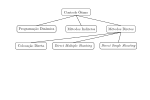
\includegraphics{DescricaoProcesso/Figuras/diagrama_metodos_numericos.png}
	\caption*{\footnotesize Fonte: Adaptado de \citeauthor{article:Diehl}}
\end{figure}

\cite{phd:Matthias} \cite{phd:Rieck} \cite{manual:Falcon}

\clearpage
\chapter{Metodologia}
\label{chap:metodologia}
\thispagestyle{empty}

\section{Definição do problema}

\section{Solução Numérica}

\subsection{\textit{FALCON.m}}

\textit{FALCON.m} é um biblioteca de \textit{MATLAB}\textsuperscript{\textregistered}, orientada a objetos, desenvolvida no \textit{Institute of Flight System Dynamics} da \textit{Technische Universit{\"a}t M{\"u}nchen} para resolução e análise de problemas de controle ótimo utilizando \cite{manual:Falcon}.



Na utilização do \textit{FALCON.m} para resolver um problema de controle ótimo são realizadas as seguintes etapas \cite{phd:Matthias}:

\begin{enumerate}
    \item \textbf{Implementar os modelos dinâmicos:} o modelo dinâmico do sistema deve ser implementado em funções do \textit{MATLAB}\textsuperscript{\textregistered}. 
    \item \textbf{Construir os modelos dinâmicos gerais dos subsistemas:} utilizar o e \textit{Model Builder} do \textit{FALCON.m} para relacionar os modelos dinâmicos nas diferentes fases do OCP.
    \item \textbf{Derivar automaticamente todas as funções necessária:} o \textit{Model Builder}irá criar, automaticamente, as derivadas analíticas de todos os subsistemas e combiná-los ao gradiente geral dos modelos usando a regra da cadeia.
    \item \textbf{Gerar código automaticamente para os modelos e compilar:}
    \item \textbf{Implementar funções de restrição adicionais:} repetir os passos de 1 à 4 para todas as restrições e funções de custo.
    \item \textbf{Definir a estrutura do problema de controle ótimo:}
    \item \textbf{Discretizar o problema de controle ótimo:}
    \item \textbf{Resolver o problema discretizado:} o problema de otimização numérica resultante da discretização do problema de controle ótimo é resolvido usando um solucionador numérico apropriado (\textit{IPOPT}, \textit{SNOPT}, \textit{FMINCON} ou \textit{WORHP}).
    \item \textbf{Analisar dos resultados:}
\end{enumerate}

Detalhes sobre o uso do \textit{FALCON.m} pode ser encontrados em sua documentação \cite{manual:Falcon}, bem com uma explicação detalhada da sua implementação na tese de doutorado de \citeauthor{phd:Rieck}.


Esse é um teste de como escreve codigo  \lstinline[style=Matlab-editor]{Bake()}

\clearpage
\chapter{Resultados}
\label{chap:resultados}

Os resultados obtidos com o desenvolvimento desse projeto são apresentados e discutidos nesse capítulo de forma divida em três seções.  
A primeira e a segunda sobre os modelos do DT1 e da pista do Kartódromo de Sonoma. E a última  sobre os resultados da solução do OCP proposto.

\section{Modelo do veículo DT1}
\label{sec:resultados_modelo}

O modelo obtido para o veículo para o veículo DT1 foi a Equação (\ref{eq:modelo_1}) e o conjunto de constates da Tabela \ref{tab:constantes}.
Entretanto esse modelo não foi validado experimentalmente pois esse projeto foi realizado, em sua maior parte, durante o regime de ensino remoto
emergência causado pela pandemia de Covid-19 em 2020. Na solução do OCP proposto a marca de consumo calculado para a estratégia ótima
foi de $905,7$ [km/kWh] que é um valor muito distante das marcas realmente realizas pelo DT1 de $266,5$ [km/kWh] em 2018 e de $226,9$ [km/kWh] em 2019  no Kartódromo de Sonoma na Shell Eco-marathon Americas. 
Apesar de que uma melhora na marca era esperada, esta grande diferença entre os valores das marcas deve ser analisada com ceticismo, ela indica que as constantes do modelo podem precisar ser ajustadas e/ou as simplificações revistas.


\section{Modelo da pista}
\label{sec:resultados_pista}

A curva ajustada para representar a altitude relativa em função da distância  apresentou um erro maior nos pontos que a distância  percorrida esta entre 290 e 575 e metros e entre 1005 e 1265 metros. O máximo erro destes
intervalos foi de 19\% e 34\% respetivamente. Ja no restante do intervalo o erro máximo ficou abaixo de 10\%. 
O modelo de inclinação, obtido a partir do arco  tangente da derivada desta curva, foi aprestando na Equação (\ref{eq:modeloTheta}). 
A Figura \ref{graf:modelo_pista} apresenta uma comparação entre os dados de altitude e a curva ajusta.
e o comportamento periódico desejado na curva ajustada para descrever a repetição das voltas na tentativa.

\begin{figure}[h]
    \centering
    \caption{Curva ajustada para representar altitude da pista}
    \input{Resultados/Figuras/pista.tex}
    \label{graf:modelo_pista}
    \caption*{\footnotesize{Fonte: Elaborada pelo autor.}}
\end{figure}


% \begin{figure}[H]
%     \centering
%     \caption{Curva ajustada para representar altitude da pista}
%     \input{Resultados/Figuras/pista_modelo.tex}
%     \label{graf:modelo_pista}
%     \caption*{\footnotesize{Fonte: Elaborada pelo autor.}}
% \end{figure}

% \begin{figure}[H]
%     \centering
%     \caption{Representação da periodicidade da curva ajusta}
%     % This file was created by matlab2tikz.
%
%The latest updates can be retrieved from
%  http://www.mathworks.com/matlabcentral/fileexchange/22022-matlab2tikz-matlab2tikz
%where you can also make suggestions and rate matlab2tikz.
%
\definecolor{mycolor1}{rgb}{0.00000,0.44700,0.74100}%
%
\begin{tikzpicture}[scale=0.85]

\begin{axis}[%
width=4.521in,
height=3.566in,
at={(0.758in,0.481in)},
scale only axis,
xmin=0,
xmax=10080,
xlabel style={font=\color{white!15!black}},
xlabel={Distancia percorrida [m]},
ymin=-2,
ymax=5,
ylabel style={font=\color{white!15!black}},
ylabel={Altitude da pista [m]},
axis background/.style={fill=white},
xmajorgrids,
ymajorgrids,
legend style={legend cell align=left, align=left, draw=white!15!black}
]
\addplot [color=mycolor1]
  table[row sep=crcr]{%
1	-0.109711917352081\\
11	-0.00839975833814072\\
21	0.0950935994183011\\
31	0.197575097473076\\
41	0.295906341954157\\
51	0.387379176406482\\
61	0.470078639152616\\
71	0.543194918667103\\
81	0.607248810660309\\
91	0.664201673014787\\
101	0.717430477656014\\
111	0.771560468559376\\
121	0.832161105813\\
131	0.90532420971175\\
141	0.997155276962692\\
151	1.11321865673269\\
161	1.25798366412261\\
171	1.43432106813152\\
181	1.64309736617324\\
191	1.88290788488262\\
201	2.14997946131707\\
211	2.43826005992245\\
221	2.73969727047449\\
231	3.04469152045332\\
241	3.34269442603896\\
251	3.62290937310388\\
261	3.87504138340178\\
271	4.09003753619072\\
281	4.26075828112619\\
291	4.38252407940657\\
301	4.45349069459108\\
311	4.47481944853005\\
321	4.45062481979224\\
331	4.38769956903536\\
341	4.29503563665075\\
351	4.18317584164875\\
361	4.06344547969927\\
371	3.94712305498246\\
381	3.84461469530785\\
391	3.76469681065797\\
401	3.71388623172202\\
411	3.69598683386881\\
421	3.71184736196174\\
431	3.75934802063559\\
441	3.83361482784037\\
451	3.92744231294103\\
461	4.03188842668885\\
471	4.13699192257323\\
481	4.23255310092945\\
491	4.30891444440015\\
501	4.35767864845305\\
511	4.37230773581937\\
521	4.34855776398591\\
531	4.28471812059516\\
541	4.18164127523908\\
551	4.04256664568099\\
561	3.8727594054464\\
571	3.6790001416205\\
581	3.46897299806302\\
591	3.25060734872116\\
601	3.03143056535272\\
611	2.81798693557988\\
621	2.61537055476623\\
631	2.42690877308266\\
641	2.25401858405504\\
651	2.09624249436254\\
661	1.95145434447245\\
671	1.81621068151138\\
681	1.68621091627265\\
691	1.55682067929601\\
701	1.42360824671759\\
711	1.28284396176586\\
721	1.13191714177985\\
731	0.969633539600276\\
741	0.796368175204486\\
751	0.614062149913995\\
761	0.426066616015826\\
771	0.236851065707892\\
781	0.051605264766321\\
791	-0.124226585294145\\
801	-0.28543530967372\\
811	-0.427514275401029\\
821	-0.547062158447048\\
831	-0.642084803994541\\
841	-0.712169858877593\\
851	-0.758519932931108\\
861	-0.783843217554211\\
871	-0.792113527366725\\
881	-0.788223438901982\\
891	-0.777563525199437\\
901	-0.765566810209672\\
911	-0.757259984130101\\
921	-0.756861473257333\\
931	-0.767461349089345\\
941	-0.790809830657308\\
951	-0.827230601643877\\
961	-0.875663350222557\\
971	-0.933827967298308\\
981	-0.998491826252851\\
991	-1.06581252391888\\
1001	-1.13172219610016\\
1011	-1.19231656474594\\
1021	-1.24421244050807\\
1031	-1.28484137061795\\
1041	-1.31265404530945\\
1051	-1.32721924116057\\
1061	-1.32921157058291\\
1071	-1.32029309615128\\
1081	-1.30290391790131\\
1091	-1.27998520033189\\
1101	-1.25466400050152\\
1111	-1.22993216571023\\
1121	-1.20835126193031\\
1131	-1.19181206044295\\
1141	-1.18137094078277\\
1151	-1.17717731518708\\
1161	-1.17849669058402\\
1171	-1.18382421671065\\
1181	-1.19107449731941\\
1191	-1.19782596034705\\
1201	-1.20159292065635\\
1211	-1.20009611694053\\
1221	-1.19150317027772\\
1231	-1.17461400061693\\
1241	-1.14897236222076\\
1251	-1.11489268027755\\
1261	-1.07340046056913\\
1271	-1.02609376840127\\
1281	-0.974941685251106\\
1291	-0.922042386510245\\
1301	-0.869367844030426\\
1311	-0.818523683801552\\
1321	-0.770551248021045\\
1331	-0.725794552227129\\
1341	-0.683848015544151\\
1351	-0.643592252309563\\
1361	-0.603315711498686\\
1371	-0.560910505351947\\
1381	-0.514122357766729\\
1391	-0.460828114779785\\
1401	-0.399310403671038\\
1411	-0.328498261776184\\
1421	-0.248145037368798\\
1431	-0.158920426954973\\
1441	-0.0624016779830519\\
1451	0.0390409958153942\\
1461	0.142458819696212\\
1471	0.244621962609591\\
1481	0.342373910009698\\
1491	0.433009194713195\\
1501	0.514636725900871\\
1511	0.586490261571256\\
1521	0.649150627850389\\
1531	0.70465094198183\\
1541	0.756445837883422\\
1551	0.809237707503833\\
1561	0.868666201312164\\
1571	0.940880473947201\\
1581	1.03202567577401\\
1591	1.14768481484112\\
1601	1.29232337115105\\
1611	1.46878624345062\\
1621	1.67789440831694\\
1631	1.91818212523839\\
1641	2.1858050795613\\
1651	2.4746363321751\\
1661	2.7765514538704\\
1671	3.0818880808922\\
1681	3.38004974341147\\
1691	3.66021056250047\\
1701	3.91206749718755\\
1711	4.12658119495929\\
1721	4.29664574188969\\
1731	4.41763189133126\\
1741	4.48775740399173\\
1751	4.50825126801585\\
1761	4.48329473066804\\
1771	4.41973993115163\\
1781	4.32662498083452\\
1791	4.21452106172837\\
1801	4.09476107417914\\
1811	3.97860935253988\\
1821	3.87643710676308\\
1831	3.79696807207257\\
1841	3.74665334488901\\
1851	3.72922399418815\\
1861	3.7454556265135\\
1871	3.7931618592856\\
1881	3.86741507237606\\
1891	3.96097443033605\\
1901	4.06488454615074\\
1911	4.16919468741892\\
1921	4.26373922867053\\
1931	4.33891587951821\\
1941	4.38639938307744\\
1951	4.3997347376935\\
1961	4.3747649568976\\
1971	4.30986296522801\\
1981	4.20595414475607\\
1991	4.06633382285708\\
2001	3.89630109056\\
2011	3.70264530253945\\
2021	3.49303317666715\\
2031	3.27535163586291\\
2041	3.05706386130738\\
2051	2.84463333293164\\
2061	2.64306324088849\\
2071	2.45558728891871\\
2081	2.28353364450786\\
2091	2.12636792910063\\
2101	1.98190511329033\\
2111	1.84666540848799\\
2121	1.7163370160708\\
2131	1.58629994863694\\
2141	1.45216078056107\\
2151	1.31024842651069\\
2161	1.15802577978455\\
2171	0.994380758508237\\
2181	0.819772148019413\\
2191	0.63621946571085\\
2201	0.447140621642194\\
2211	0.257055072709677\\
2221	0.0711822165349781\\
2231	-0.105026119306842\\
2241	-0.266374844844081\\
2251	-0.408390936247001\\
2261	-0.52772236817059\\
2271	-0.622434877067988\\
2281	-0.692180725667297\\
2291	-0.738225775326999\\
2301	-0.763334352315229\\
2311	-0.771524388431763\\
2321	-0.767716935020035\\
2331	-0.757313347586203\\
2341	-0.745739411463418\\
2351	-0.737997933651879\\
2361	-0.7382697204275\\
2371	-0.749597612541098\\
2381	-0.773679911866189\\
2391	-0.810788934937414\\
2401	-0.859818595970919\\
2411	-0.918452978348607\\
2421	-0.9834369141028\\
2431	-1.05092065765553\\
2441	-1.11684460981355\\
2451	-1.17732724078422\\
2461	-1.22902007508595\\
2471	-1.26939769943262\\
2481	-1.29695778207113\\
2491	-1.31131532379874\\
2501	-1.31318587487361\\
2511	-1.30426321938879\\
2521	-1.28700701334462\\
2531	-1.26436412045858\\
2541	-1.23945315760302\\
2551	-1.21524452852757\\
2561	-1.19426777701328\\
2571	-1.17837453046989\\
2581	-1.1685790351634\\
2591	-1.16498996650145\\
2601	-1.16683768558383\\
2611	-1.17259136664965\\
2621	-1.18015141108624\\
2631	-1.18709518087878\\
2641	-1.19094904643271\\
2651	-1.18945752987899\\
2661	-1.18082112945581\\
2671	-1.163878124775\\
2681	-1.13821188746484\\
2691	-1.10417330744339\\
2701	-1.06281705745925\\
2711	-1.01575962122082\\
2721	-0.964975358495653\\
2731	-0.912553514665536\\
2741	-0.860443314589362\\
2751	-0.810215664323673\\
2761	-0.762868359004461\\
2771	-0.71869720512976\\
2781	-0.677248546929054\\
2791	-0.637360026867475\\
2801	-0.597286881858604\\
2811	-0.554901651476558\\
2821	-0.507946828414134\\
2831	-0.454313597483903\\
2841	-0.392316088042783\\
2851	-0.32092995139631\\
2861	-0.239966711702738\\
2871	-0.150161045476146\\
2881	-0.0531564291649808\\
2891	0.0486153042655554\\
2901	0.152154000824888\\
2911	0.254193570256236\\
2921	0.351560026288614\\
2931	0.441551312851706\\
2941	0.522300934601968\\
2951	0.593086875477846\\
2961	0.654550515125696\\
2971	0.708797066931038\\
2981	0.759358941488504\\
2991	0.811015556340023\\
3001	0.869476400370953\\
3011	0.940947410493913\\
3021	1.03161268752164\\
3031	1.14707310812312\\
3041	1.29178951328604\\
3051	1.46858018988898\\
3061	1.67821998581917\\
3071	1.91918167958509\\
3081	2.18754962831664\\
3091	2.47712207229177\\
3101	2.77970290432061\\
3111	3.08556754338769\\
3121	3.38407219379886\\
3131	3.66436259362606\\
3141	3.91612856605821\\
3151	4.13034521696469\\
3161	4.29994104254356\\
3171	4.42033767516037\\
3181	4.48981521803792\\
3191	4.50967039565048\\
3201	4.48415100883931\\
3211	4.42016809033865\\
3221	4.32680520673144\\
3231	4.21466101621697\\
3241	4.09507504098498\\
3251	3.97929645047824\\
3261	3.87766061455082\\
3271	3.79883782313765\\
3281	3.74921288521327\\
3291	3.73244377411941\\
3301	3.74923295617508\\
3311	3.79732774518316\\
3321	3.87174742517548\\
3331	3.96521654733918\\
3341	4.06876728002307\\
3351	4.17246036019907\\
3361	4.26616516957475\\
3371	4.34033547371321\\
3381	4.38671871661783\\
3391	4.39894329435757\\
3401	4.37293933330678\\
3411	4.3071631763426\\
3421	4.20261273892485\\
3431	4.06263865658181\\
3441	3.89257317190016\\
3451	3.69921354891173\\
3461	3.49020820883375\\
3471	3.27340082063725\\
3481	3.05618971294326\\
3491	2.84495709652224\\
3501	2.64461503596073\\
3511	2.45830362736606\\
3521	2.28726250410126\\
3531	2.1308809180206\\
3541	1.98691565929691\\
3551	1.8518514011584\\
3561	1.72136596576967\\
3571	1.59085453256746\\
3581	1.45596263994659\\
3591	1.31307825849592\\
3601	1.15973811531745\\
3611	0.994912300750151\\
3621	0.819143120439789\\
3631	0.634528032965973\\
3641	0.444551044677242\\
3651	0.253780789344372\\
3661	0.067465453952224\\
3671	-0.108936328528585\\
3681	-0.270244277566914\\
3691	-0.412019541837268\\
3701	-0.530959746561425\\
3711	-0.625190629127377\\
3721	-0.694428927063916\\
3731	-0.740003375712762\\
3741	-0.764733857930665\\
3751	-0.772681697365916\\
3761	-0.768795614412628\\
3771	-0.758486934206376\\
3781	-0.747173456839254\\
3791	-0.739833492203418\\
3801	-0.740609799003622\\
3811	-0.752497782021677\\
3821	-0.777143858212993\\
3831	-0.814769239760178\\
3841	-0.864222532183184\\
3851	-0.923152632602985\\
3861	-0.988282548629893\\
3871	-1.05575593642078\\
3881	-1.12152216306434\\
3891	-1.18172304029534\\
3901	-1.2330452376257\\
3911	-1.27300661210768\\
3921	-1.30015182191712\\
3931	-1.31414188744043\\
3941	-1.31573289867114\\
3951	-1.30664981102404\\
3961	-1.2893711898497\\
3971	-1.26684891960167\\
3981	-1.24219253384207\\
3991	-1.21835044847344\\
4001	-1.1978197932734\\
4011	-1.18241285119381\\
4021	-1.17310174602351\\
4031	-1.16995463817434\\
4041	-1.17216715502379\\
4051	-1.17818305848217\\
4061	-1.18588920790449\\
4071	-1.19286259337564\\
4081	-1.19664230167593\\
4091	-1.19499720194536\\
4101	-1.1861610808664\\
4111	-1.16901079597025\\
4121	-1.14316933894755\\
4131	-1.10902384946087\\
4141	-1.0676577531166\\
4151	-1.02070537634236\\
4161	-0.970145672985785\\
4171	-0.918058229257204\\
4181	-0.866368817033628\\
4191	-0.816613005865686\\
4201	-0.769744574766057\\
4211	-0.726010844066624\\
4221	-0.684910024423064\\
4231	-0.645236952226242\\
4241	-0.605214027510975\\
4251	-0.562694766890764\\
4261	-0.515419104674251\\
4271	-0.461293297230767\\
4281	-0.398663699763548\\
4291	-0.326553224018508\\
4301	-0.244832078074922\\
4311	-0.154300239894579\\
4321	-0.0566675192038929\\
4331	0.0455727546647442\\
4341	0.149369386827174\\
4351	0.251420549341063\\
4361	0.348535438860226\\
4371	0.43801613507362\\
4381	0.518021462428984\\
4391	0.587874283886948\\
4401	0.648277049708184\\
4411	0.701407398116836\\
4421	0.750875621708201\\
4431	0.801538031519352\\
4441	0.859173593767532\\
4451	0.930044467953282\\
4461	1.02037299678602\\
4471	1.13577713279455\\
4481	1.28071227468474\\
4491	1.45796935967078\\
4501	1.66827650581806\\
4511	1.91004460591045\\
4521	2.17928652306115\\
4531	2.46972577130372\\
4541	2.77309491764668\\
4551	3.07960774777241\\
4561	3.37857390822608\\
4571	3.65911164116987\\
4581	3.9109045630591\\
4591	4.12494312733209\\
4601	4.29419101003624\\
4611	4.41412130287145\\
4621	4.48307678853789\\
4631	4.50242198846714\\
4641	4.47647103250519\\
4651	4.41219335336525\\
4661	4.31871725034078\\
4671	4.20666796676953\\
4681	4.0873906626068\\
4691	3.97211834925178\\
4701	3.87114963927479\\
4711	3.79310061457673\\
4721	3.74428925339168\\
4731	3.72830015534106\\
4741	3.74576265609394\\
4751	3.79435806025612\\
4761	3.86905310750416\\
4771	3.96253849399793\\
4781	4.06583484054178\\
4791	4.16901530948211\\
4801	4.26198522019608\\
4811	4.33525521774953\\
4821	4.38064609247041\\
4831	4.39187005086318\\
4841	4.36494447888093\\
4851	4.29840900944683\\
4861	4.1933337038751\\
4871	4.05312389808791\\
4881	3.88314421678459\\
4891	3.69019897482842\\
4901	3.48191742914298\\
4911	3.26609919799272\\
4921	3.05007710428843\\
4931	2.84015163896252\\
4941	2.64114353254819\\
4951	2.45609932428189\\
4961	2.28617041640072\\
4971	2.13067021610322\\
4981	1.98729802936202\\
4991	1.85250379249395\\
5001	1.72195577913788\\
5011	1.59106511764574\\
5021	1.45551697068141\\
5031	1.31175884148751\\
5041	1.15740153965532\\
5051	0.99149732503302\\
5061	0.814671769383148\\
5071	0.629099789858731\\
5081	0.438330822075135\\
5091	0.246981886079804\\
5101	0.0603291160437442\\
5111	-0.116162866917553\\
5121	-0.277329310060742\\
5131	-0.418766089329753\\
5141	-0.537220822197283\\
5151	-0.630879345724785\\
5161	-0.699522720430722\\
5171	-0.744542168499829\\
5181	-0.768812543414552\\
5191	-0.77643783019091\\
5201	-0.772393610273662\\
5211	-0.76210036636017\\
5221	-0.750967170276958\\
5231	-0.743947226880766\\
5241	-0.745144827455544\\
5251	-0.757507744184746\\
5261	-0.782630549922456\\
5271	-0.820683622954029\\
5281	-0.870470731289588\\
5291	-0.929606210591703\\
5301	-0.99479196170474\\
5311	-1.06216578441959\\
5321	-1.12768670827949\\
5331	-1.18752047223153\\
5341	-1.23838931245838\\
5351	-1.27785457667711\\
5361	-1.30450791418447\\
5371	-1.31805615030916\\
5381	-1.31929550819321\\
5391	-1.30998155813075\\
5401	-1.29261112467127\\
5411	-1.27014043391958\\
5421	-1.24566929528688\\
5431	-1.22212359738301\\
5441	-1.20196767103155\\
5451	-1.18697426226862\\
5461	-1.17807339173284\\
5471	-1.17529293472056\\
5481	-1.17779420370248\\
5491	-1.18399611608134\\
5501	-1.19177265158176\\
5511	-1.19870112164413\\
5521	-1.20233398658379\\
5531	-1.20046501983181\\
5541	-1.19136169939746\\
5551	-1.17393966917773\\
5561	-1.14786153323961\\
5571	-1.11355045593862\\
5581	-1.07211819273916\\
5591	-1.02521633013662\\
5601	-0.974827727368291\\
5611	-0.923021580649208\\
5621	-0.871699504103512\\
5631	-0.822361118090603\\
5641	-0.775915722528825\\
5651	-0.732561882075727\\
5661	-0.691749623454086\\
5671	-0.65223115090478\\
5681	-0.612196409817006\\
5691	-0.569480448737413\\
5701	-0.521821319121635\\
5711	-0.467141081524286\\
5721	-0.403819037629839\\
5731	-0.330926000139338\\
5741	-0.248391360738889\\
5751	-0.157080710186729\\
5761	-0.0587702847557871\\
5771	0.0439852237341798\\
5781	0.148083927953945\\
5791	0.250188792131437\\
5801	0.347092856381779\\
5811	0.436103063773211\\
5821	0.515404282722282\\
5831	0.584364905130815\\
5841	0.643748963145229\\
5851	0.695806840655715\\
5861	0.744226808470209\\
5871	0.793941929590395\\
5881	0.850800277683937\\
5891	0.921119667893307\\
5901	1.011159971315\\
5911	1.12655542147619\\
5921	1.271755172588\\
5931	1.44952207862169\\
5941	1.66053693379028\\
5951	1.90314834984942\\
5961	2.17329754111752\\
5971	2.46463340145052\\
5981	2.76881753564511\\
5991	3.07600269022259\\
6001	3.37545273019981\\
6011	3.656259294355\\
6021	3.9081007238689\\
6031	4.12198370809991\\
6041	4.29090786883547\\
6051	4.41039833106196\\
6061	4.47886088571468\\
6071	4.49772790263973\\
6081	4.471379606938\\
6091	4.40684332952534\\
6101	4.31329137350302\\
6111	4.20137467243125\\
6121	4.08244303908869\\
6131	3.96771233603063\\
6141	3.8674435067867\\
6151	3.79019767061393\\
6161	3.74222544191348\\
6171	3.72703777993521\\
6181	3.74519091099121\\
6191	3.79430043593274\\
6201	3.86928111097238\\
6211	3.96279054259811\\
6221	4.06583870523537\\
6231	4.16851214344749\\
6241	4.26075304238937\\
6251	4.3331297448767\\
6261	4.37753702534393\\
6271	4.38777130422695\\
6281	4.35993736394961\\
6291	4.29265798971039\\
6301	4.1870749929942\\
6311	4.04664779638075\\
6321	3.87677263408077\\
6331	3.68426001332165\\
6341	3.47671916247087\\
6351	3.26190485882661\\
6361	3.04708377558004\\
6371	2.83847424421572\\
6381	2.6408054648315\\
6391	2.45703048271724\\
6401	2.28821278321631\\
6411	2.13359046321988\\
6421	1.99080604758482\\
6431	1.85627554080943\\
6441	1.72565849925616\\
6451	1.59438277965339\\
6461	1.45817382375786\\
6471	1.31353913658475\\
6481	1.15816384991459\\
6491	0.991182380977039\\
6501	0.813303304567194\\
6511	0.626778506348153\\
6521	0.4352221789461\\
6531	0.243298935633004\\
6541	0.0563120162181395\\
6551	-0.120268783558876\\
6561	-0.281294950527896\\
6571	-0.42239763380241\\
6581	-0.540374774359932\\
6591	-0.633472396556515\\
6601	-0.70153572122028\\
6611	-0.746018060524634\\
6621	-0.769848644848614\\
6631	-0.77717338488352\\
6641	-0.77299391283215\\
6651	-0.762739057602265\\
6661	-0.751808423263048\\
6671	-0.745129507602381\\
6681	-0.746767722214123\\
6691	-0.759623018490201\\
6701	-0.785238174383896\\
6711	-0.823733012168367\\
6721	-0.87386693919754\\
6731	-0.93322035773951\\
6741	-0.998474779967866\\
6751	-1.06576288867175\\
6761	-1.13105406663915\\
6771	-1.19053855787688\\
6781	-1.24097457724413\\
6791	-1.27996717273519\\
6801	-1.30615497509042\\
6811	-1.31929038980985\\
6821	-1.32020935804754\\
6831	-1.31069750224054\\
6841	-1.29326925241673\\
6851	-1.27088449661721\\
6861	-1.24663268151009\\
6871	-1.22341663376531\\
6881	-1.20366750708417\\
6891	-1.18911832614556\\
6901	-1.18065703615198\\
6911	-1.17827146502713\\
6921	-1.18108903564423\\
6931	-1.18750439313141\\
6941	-1.19537930179836\\
6951	-1.20229208664139\\
6961	-1.20580923474658\\
6971	-1.20374997459447\\
6981	-1.19441586979588\\
6991	-1.17676154907852\\
7001	-1.15048921068425\\
7011	-1.1160578084506\\
7021	-1.07460699575215\\
7031	-1.02780502950524\\
7041	-0.977637981160131\\
7051	-0.926163924454248\\
7061	-0.875259612208226\\
7071	-0.826388106781589\\
7081	-0.780413772084764\\
7091	-0.737486155146442\\
7101	-0.697007056617631\\
7111	-0.657686230503229\\
7121	-0.617681556658883\\
7131	-0.574810175445773\\
7141	-0.526808933487088\\
7151	-0.471616427767162\\
7161	-0.407645623721687\\
7171	-0.334015869348012\\
7181	-0.250716231079849\\
7191	-0.158678213566937\\
7201	-0.0597445617627375\\
7211	0.0434688150042029\\
7221	0.147809695550517\\
7231	0.249906374477391\\
7241	0.346536401770879\\
7251	0.435012314442613\\
7261	0.513545748882924\\
7271	0.58155127266305\\
7281	0.639855005254393\\
7291	0.690780389188819\\
7301	0.738093760638044\\
7311	0.786804783693372\\
7321	0.842830260918894\\
7331	0.912543089050261\\
7341	1.00223994928583\\
7351	1.11757055938818\\
7361	1.26297702811862\\
7371	1.44119339704165\\
7381	1.65285254976734\\
7391	1.89624043131084\\
7401	2.16722646355438\\
7411	2.45938503801703\\
7421	2.76430717231811\\
7431	3.07208517813766\\
7441	3.37193792328874\\
7451	3.6529313410688\\
7461	3.90473943112655\\
7471	4.11838600618794\\
7481	4.28690739578024\\
7491	4.40588132572593\\
7501	4.47377691574696\\
7511	4.49209442642569\\
7521	4.46527993526424\\
7531	4.400418161491\\
7541	4.30672467685665\\
7551	4.19487520652659\\
7561	4.07622323047485\\
7571	3.9619664741243\\
7581	3.86232730580276\\
7591	3.78581113579335\\
7601	3.73860069188631\\
7611	3.72413303781792\\
7621	3.74289132358689\\
7631	3.79242576274579\\
7641	3.86759969829595\\
7651	3.96103841935221\\
7661	4.06374215910588\\
7671	4.16581180191836\\
7681	4.25722732434861\\
7691	4.3286155798219\\
7701	4.37194595695006\\
7711	4.38109948435756\\
7721	4.35226846800225\\
7731	4.2841586981622\\
7741	4.17798333274786\\
7751	4.03725526139993\\
7761	3.86740155221951\\
7771	3.67523804653447\\
7781	3.46835308341198\\
7791	3.25445581554871\\
7801	3.04074613164843\\
7811	2.83335977527225\\
7821	2.63693423183279\\
7831	2.45432912774566\\
7841	2.28652035687543\\
7851	2.13267124948148\\
7861	1.99036825914209\\
7871	1.85599426732478\\
7881	1.72520094479848\\
7891	1.59343365339373\\
7901	1.45645876325882\\
7911	1.31084424261564\\
7921	1.15434977611166\\
7931	0.986191916808387\\
7941	0.807161970594909\\
7951	0.619588294202077\\
7961	0.427149159872773\\
7971	0.234555978707817\\
7981	0.0471382553501445\\
7991	-0.129629849521732\\
8001	-0.290616767448686\\
8011	-0.431489457692471\\
8021	-0.549096505539075\\
8031	-0.64174419916296\\
8041	-0.709341746213374\\
8051	-0.753404142381356\\
8061	-0.776914393574985\\
8071	-0.78405959540548\\
8081	-0.779866618407227\\
8091	-0.769771827220102\\
8101	-0.759164622340435\\
8111	-0.752946198467872\\
8121	-0.755142682906191\\
8131	-0.768606026551919\\
8141	-0.794827270057781\\
8151	-0.833875964981332\\
8161	-0.884467640493358\\
8171	-0.944149396724428\\
8181	-1.00958307563319\\
8191	-1.07689697975942\\
8201	-1.14207153047971\\
8211	-1.20132204683009\\
8221	-1.25144312467191\\
8231	-1.29008371120361\\
8241	-1.3159293981306\\
8251	-1.32877793633509\\
8261	-1.32950456143636\\
8271	-1.31992437914831\\
8281	-1.30256876786739\\
8291	-1.2804005974098\\
8301	-1.25649831553355\\
8311	-1.23374115727839\\
8321	-1.21452672796891\\
8331	-1.20054815460003\\
8341	-1.19265134310186\\
8351	-1.19078431965754\\
8361	-1.19404104934135\\
8371	-1.20079248162257\\
8381	-1.20888883138123\\
8391	-1.21591012826711\\
8401	-1.21943753540864\\
8411	-1.21731628054999\\
8421	-1.20788239857789\\
8431	-1.19012969157679\\
8441	-1.16379992332827\\
8451	-1.12938759190208\\
8461	-1.08805980784403\\
8471	-1.04150090203569\\
8481	-0.991699460684102\\
8491	-0.940701701124891\\
8501	-0.890358812759513\\
8511	-0.842096695216966\\
8521	-0.796734325721692\\
8531	-0.754371979419795\\
8541	-0.714363197083409\\
8551	-0.675375472459833\\
8561	-0.635535015902263\\
8571	-0.59264162446658\\
8581	-0.544431620444267\\
8591	-0.488860869090527\\
8601	-0.42437671347977\\
8611	-0.350147665068909\\
8621	-0.266222947654343\\
8631	-0.173600270670087\\
8641	-0.0741889588387081\\
8651	0.029334016950841\\
8661	0.133766470226962\\
8671	0.235702572313187\\
8681	0.331905055122274\\
8691	0.419692782874768\\
8701	0.497304883520215\\
8711	0.564202743597134\\
8721	0.62127506928774\\
8731	0.670918666695638\\
8741	0.716978015286696\\
8751	0.764539219899451\\
8761	0.819587424681491\\
8771	0.888550026756298\\
8781	0.977759794334847\\
8791	1.09288113073782\\
8801	1.23834829957129\\
8811	1.41686580522804\\
8821	1.62901804120995\\
8831	1.87302790960728\\
8841	2.14469290726212\\
8851	2.43751305283213\\
8861	2.74300916305842\\
8871	3.05121372906064\\
8881	3.35130141361612\\
8891	3.63231334755117\\
8901	3.88392012472716\\
8911	4.0971635675009\\
8921	4.26511747098089\\
8931	4.38341272272904\\
8941	4.45058208338723\\
8951	4.46819373728526\\
8961	4.44075936223278\\
8971	4.37542054766766\\
8981	4.28143539250787\\
8991	4.16950351116048\\
9001	4.05098106444816\\
9011	3.9370466548522\\
9021	3.8378831748886\\
9031	3.76193958774887\\
9041	3.71533022204889\\
9051	3.70141800223998\\
9061	3.72061304662164\\
9071	3.77040050869587\\
9081	3.84559289760919\\
9091	3.93878396405898\\
9101	4.04096510882081\\
9111	4.1422525140611\\
9121	4.23266487057928\\
9131	4.30288834959105\\
9141	4.34496757598024\\
9151	4.35286857134679\\
9161	4.32287128222323\\
9171	4.25376434719113\\
9181	4.14683185865955\\
9191	4.00563954778157\\
9201	3.8356445378355\\
9211	3.64366714612535\\
9221	3.43727396512377\\
9231	3.22412774583121\\
9241	3.0113609668279\\
9251	2.80502636626579\\
9261	2.60966954257118\\
9271	2.42805679028131\\
9281	2.26107674811657\\
9291	2.10781853241108\\
9301	1.96581324173337\\
9311	1.83141144666797\\
9321	1.70025776416936\\
9331	1.56781583483287\\
9341	1.42989360066487\\
9351	1.28311994656556\\
9361	1.12532933146248\\
9371	0.955820413072912\\
9381	0.775466947419435\\
9391	0.586673257344062\\
9401	0.393181012063504\\
9411	0.199747622672146\\
9421	0.0117280184922139\\
9431	-0.165400080810512\\
9441	-0.326522750100184\\
9451	-0.467343286995707\\
9461	-0.584761231633036\\
9471	-0.677143201659642\\
9481	-0.744462207517106\\
9491	-0.78829451263121\\
9501	-0.811676289767742\\
9511	-0.818835073994697\\
9521	-0.814822159982188\\
9531	-0.805080638858982\\
9541	-0.794988975757328\\
9551	-0.7894214726074\\
9561	-0.792364575784742\\
9571	-0.806622064732274\\
9581	-0.833633309021319\\
9591	-0.873417882386367\\
9601	-0.924647924063045\\
9611	-0.984837866629531\\
9621	-1.05063060077145\\
9631	-1.11815078304702\\
9641	-1.18339055345956\\
9651	-1.2425908683301\\
9661	-1.2925830973638\\
9671	-1.33106027543809\\
9681	-1.35675492421612\\
9691	-1.36950989546535\\
9701	-1.37023928765588\\
9711	-1.36078711515073\\
9721	-1.34370104459822\\
9731	-1.32194624736828\\
9741	-1.29858953894479\\
9751	-1.27648603836314\\
9761	-1.25799943856238\\
9771	-1.24478280093972\\
9781	-1.23764003702797\\
9791	-1.23647962501759\\
9801	-1.24036251066657\\
9811	-1.24763652895464\\
9821	-1.25614101324343\\
9831	-1.26345838798365\\
9841	-1.26718513781449\\
9851	-1.26519302759362\\
9861	-1.25585294076593\\
9871	-1.23819803160341\\
9881	-1.21200959064062\\
9891	-1.17781740521239\\
9901	-1.13681559386255\\
9911	-1.09070395855907\\
9921	-1.04147289893599\\
9931	-0.991156040975843\\
9941	-0.941578310392307\\
9951	-0.894127843829391\\
9961	-0.849577787757336\\
9971	-0.80797889922967\\
9981	-0.768636433971275\\
9991	-0.730175823784505\\
10001	-0.690692012705508\\
10011	-0.647968024570274\\
10021	-0.599740340505644\\
10031	-0.543982825652031\\
10041	-0.479177911405949\\
10051	-0.40454389486101\\
10061	-0.32019063148132\\
10071	-0.227182316423454\\
};
\addlegendentry{Ajuste}

%\addlegendentry{Termino da volta}

\end{axis}

\begin{axis}[%
width=5.833in,
height=4.375in,
at={(0in,0in)},
scale only axis,
xmin=0,
xmax=1,
ymin=0,
ymax=1,
axis line style={draw=none},
ticks=none,
axis x line*=bottom,
axis y line*=left
]
\end{axis}
\end{tikzpicture}%
%     \label{graf:pista_voltas}
%     \caption*{\footnotesize{Fonte: Elaborada pelo autor.}}
% \end{figure}

\section{estratégia de pista ótima}
\label{sec:resultados_otimo}
 
O código desenvolvido, conforme descrito na Seção \ref{sec:OCPporposto}, para solução o problema de controle ótimo proposto na Equação 
(\ref{eq:ObjOCP_final}) gerou um problema de programação não linear com 3005 variáveis de otimização.
Foram gastos para a execução de todo o programa $\sim 14.4$ segundos onde $\sim 7,2$ segundos deste foram utilizados na otimização do NLP em $636$ iterações da biblioteca IPOP e reposta não violou nenhuma das restrições. 
A sequência de controle ótima de $i$ e os estados gerados por ela $x$ e $v$ estão apresentados nos gráficos da Figura \ref{graf:resultadoOCP}. 
Os parâmetros otimizados tempo final $T$ e raio do eixo do motor $r_m$ são exibidos na Tabela \ref{tab:resultadoOCP} junto das métricas marca, velocidade media e velocidade final. 

\begin{table}[h]
	\centering
	\caption{Parâmetros otimizados e métricas da estratégia ótima}
	\rowcolors{1}{}{lightgray}
	\begin{tabular}{lll}
		\toprule
		\textbf{Constante} & \textbf{Unidade} & \textbf{Valor}\\
		\hline
		Marca                               & [$km/kWh$]   & 905.68  \\
        Raio do eixo do motor               & [$mm$]       & 27.56   \\
        Tempo total de prova                & [$s$]        & 1400.0  \\  
        Velocidade média                    & [$km/h$]     & 25.92   \\
        Velocidade final                    & [$km/h$ ]    & 17.09   \\
		\bottomrule
	\end{tabular}
	\caption*{\footnotesize Fonte: Elaborada pelo autor.}
	\label{tab:resultadoOCP}
\end{table}

\begin{figure}[H]
    \centering
    \caption{sequência de controle ótima $i$ e estados $v$ e $x$ correspondentes}
    \input{Resultados/Figuras/resultadoOPC.tex}
    \label{graf:resultadoOCP}
    \caption*{\footnotesize{Fonte: Elaborada pelo autor.}}
\end{figure}

A estratégia de pista ótima encontrada se assemelha muito a estratégia estratégia \textit{start-stop}, na qual o motor é desligado quando a velocidade é máxima
km/h e religado apenas quando é minima. Entretanto, no caso ótimo estes valores diferem na primeira, na última e nas demais voltas. Para a primeira volta a máxima e a mínima são
$26,8$ e $17,3$ [km/h]. Na última  os valores máximo e a mínimo são $33,2$ e $11,9$ [km/h]. Enquanto nas demais voltas os valores máximo e mínimo são $35,0$ e $17,3$ [km/h]

Nos gráficos da Figura \ref{graf:resultadotensao} estão retratos a tensão que deve ser aplicada no motor para produzir a corrente elétrica da sequência de controle ótima e a inclinação da pista em cada instante de tempo.
A partir desta pode-se observar que o motor é ligado somente no maior pico positivo de inclinação, ou seja, o motor só é ligado na maior subida pista.

Como apresentado nos gráficos da Figura \ref{graf:resultadoForcas} a maior força resistiva que atuou no veículo foi a componente do peso paralela a pista $F_g$, variando entre $-18,45$ [N] a $25,84$ [N]. Apesar de $F_g$ ser conservativa
e realizar um trabalho nulo em um circuito fechado, ela influencia fortemente, dado sua magnitude comparada as outras forças resistivas, as acelerações do protótipo e consequentemente a região de trabalho do motor.
Já o arrasto aerodinâmico $F_a$ atingiu um máximo de $2,46$ [N] e a resistência ao rolamento $F_r$ teve o valor constante de $2,02$ [N].  

\begin{figure}[h]
    \centering
    \caption{Tensão necessária para a sequência de controle ótima e inclinação da pista}
    \input{Resultados/Figuras/resultado_tensao.tex}
    \label{graf:resultadotensao}
    \caption*{\footnotesize{Fonte: Elaborada pelo autor.}}
\end{figure}

\begin{figure}[h]
    \centering
    \caption{Força tração das forças resistivas na estratégia de pista ótima}
    \input{Resultados/Figuras/resultado_forcas.tex}
    \label{graf:resultadoForcas}
    \caption*{\footnotesize{Fonte: Elaborada pelo autor.}}
\end{figure}







\clearpage
\chapter{Conclusões}
\label{chap:conclusao}
\thispagestyle{empty}

O capítulo de conclusão deste projeto de fim de curso está divido em duas seções.
Na Seção \ref{sec:5_1} são feitas as considerações finais sobre os resultados alcançados e uma avaliação do cumprimento dos objetivos definidos inicialmente no Capítulo \ref{chap:intro}.
As propostas de continuidade para o projeto estão na Seção \ref{sec:5_2}.

\section{Considerações Finais}
\label{sec:5_1}

Os objetivos (a) e (d) de definir o modelo matemático para a dinâmica do protótipo DT1 e de definir a estratégia ótima para a pista da Shell EcoMarathon Américas de 2019 
foram atingidos de forma parcial uma vez que, como discutido na Seção \ref{sec:resultados_modelo}, não foi realizado uma validação experimental do modelo e, desta forma, não é possível afirmar que o modelo determinado representa fidedignamente o comportamento do veículo
e por consequência que a estratégia de pista e a relação de transmissão encontradas são ótimas para o caso real. Contudo foi possível obter as seguintes conclusões a partir da estrategia encontrada que 
podem ser utilizadas como orientações na realização da tentativa: 

\begin{itemize}
    \item O motor deve ser ligado no trecho de maior aclive da pista;
    \item O tempo total gasto deve ser o máximo permitido;
    \item O tempo da ultima volta é maior que o tempo das demais;
    \item A velocidade final é maior que zero.
\end{itemize}



Formular o problema de controle ótimo pra obter a estratégia ótima e implementar o algoritmo para solução desse OCP,
que são objetos (b) e (c), foram cumpridos integralmente pois a formulação contempla todas as restrições para o comportamento do veículo durante uma tentativa e o solução cumpriu todas estas
restrições com um tempo de computação pequeno. Além disso a formulação do OCP e o código serão de fácil modificação nas propostas de continuidade do trabalho
a fim de concluir os objetivos (a) e (d).

\section{Propostas de Continuidade}
\label{sec:5_2}

A principal proposta para continuidade deste projeto e evolução e validação experimental do modelo matemático do protótipo DT1.
Realizar a validação experimental é de fundamental importância para que os resultados obtidos com a solução do OCP possam ser utilizados pela equipe Milhagem UFMG.
Essa evolução deve considerar pontos como a resistência ao rolamento do pneu em curvas, o atrito viscoso dos rolamento e perdas na bateria e no conversor de potência.

Outro ponto de continuidade é a modificação do código escrito pra que a dinâmica e perdas do indutor da armadura motor sejam consideradas a fim de confirmar
se são desconsideráveis.  
Modificar, também, a restrição de caminho da corrente de forma que ela possa atingir valores maiores que o limite de $30$ [A] durante a partida para que 
seja avaliada na otimização a possibilidade de usar a corrente de pico do motor, que é de $63$ [A], para que o protótipo tenha
uma maior aceleração no momento da partida. 

\clearpage


\addcontentsline{toc}{chapter}{Referências Bibliográficas}
\renewcommand{\bibname}{Referências Bibliográficas}

\bibliographystyle{abntex2-num}
\begin{small}
\bibliography{ListadeReferencias}
\end{small}

\appendix
\chapter{Códigos implementados}

Este apêndice contém os códigos implementados pelo autor apresentados na Seção \ref{sec:metodologia_codigos}.

\lstinputlisting[
  style      = Matlab-editor,
  basicstyle = \mlttfamily\scriptsize,
  caption={[Arquivo i\_max.m]{Arquivo i\_max.m}},
]{Apendices/Codigos/i_max.m}

\lstinputlisting[
  style      = Matlab-editor,
  basicstyle = \mlttfamily\scriptsize,
  caption={[Arquivo lagrange\_cost.m]{Arquivo lagrange\_cost.m}},
]{Apendices/Codigos/LagrangeCost.m}

\lstinputlisting[
  style      = Matlab-editor,
  basicstyle = \mlttfamily\scriptsize,
  caption={[Arquivo mdl\_dt1\_pista.m]{Arquivo mdl\_dt1\_pista.m}},
]{Apendices/Codigos/mdl_dt1_pista.m}

\lstinputlisting[
  style      = Matlab-editor,
  basicstyle = \mlttfamily\scriptsize,
  caption={[Arquivo main.m]{Arquivo main.m}},
]{Apendices/Codigos/main.m}
\chapter{Dados da pista}

É apresentado na Tabela \ref{tab:Pista} o dados coletados e processados da pista da Shell Eco-marathon Americas de 2019
 no Kartódromo de Sonoma pela equipe \textit{Duke Electric Vehicles} da 
\textit{Duke University} concedidos a equipe Milhagem UFMG por meio de solicitação no site \url{http://www.duke-ev.org/}.

\rowcolors{1}{}{lightgray}
\begin{longtable}{p{2.5cm}p{2.5cm}p{3cm}p{3cm}p{2.5cm}}
    \caption{Dados da pista da Shell Eco-marathon Americas de 2019}\\
    \toprule
	\textbf{Distância percorrida [m]} & \textbf{Variação de altitude [m]} & \textbf{Latitude} & \textbf{Longitude} &\textbf{Elevação}\\
    \hline
        0	  &       0	    &               38.1612738600  &   -122.454429100   &	-21.21110 \\
        5.122  &	     0.0357 &               38.1613029200  &   -122.454474500   &	-21.17536 \\
        10.05  &	     0.1049 &               38.1613307940  &   -122.454518280   &	-21.10612 \\
        15.10  &	     0.1077 &               38.1613587920  &   -122.454563700   &	-21.10336 \\
        20.05  &	     0.1434 &               38.1613862320  &   -122.454608280   &	-21.06766 \\
        25.01  &	     0.1853 &               38.1614137920  &   -122.454652860   &	-21.02566 \\
        30.09  &	     0.2428 &               38.1614427520  &   -122.454697760   &	-20.96822 \\
        35.01  &	     0.2653 &               38.1614707900  &   -122.454741240   &	-20.94566 \\
        40.10  &	     0.3062 &               38.1614994740  &   -122.454786460   &	-20.90476 \\
        45.03  &	     0.3443 &               38.1615268620  &   -122.454830700   &	-20.86662 \\
        50.01  &	     0.3632 &               38.1615544000  &   -122.454875700   &	-20.84766 \\
        55.06  &	     0.4084 &               38.1615828700  &   -122.454920500   &	-20.80246 \\
        60.08  &	     0.4487 &               38.1616102000  &   -122.454966160   &	-20.76208 \\
        65.00  &	     0.5074 &               38.1616373020  &   -122.455010600   &	-20.70332 \\
        70.01  &	     0.5286 &               38.1616649540  &   -122.455055780   &	-20.68206 \\
        75.04  &	     0.5487 &               38.1616924220  &   -122.455101420   &	-20.66192 \\
        80.02  &	     0.5800 &               38.1617207240  &   -122.455145600   &	-20.63052 \\
        85.05  &	     0.6030 &               38.1617487200  &   -122.455190660   &	-20.60744 \\
        90.00  &	     0.6475 &               38.1617766380  &   -122.455234700   &	-20.56290 \\
        95.03  &	     0.6991 &               38.1618043860  &   -122.455280080   &	-20.51126 \\
       100.08  & 	 0.7343 &               38.1618322140  &   -122.455325660   &	-20.47594 \\
       105.08  & 	 0.7766 &               38.1618600180  &   -122.455370600   &	-20.43358 \\
       110.02  & 	 0.8014 &               38.1618862000  &   -122.455416200   &	-20.40868 \\
       115.10  & 	 0.8308 &               38.1619142460  &   -122.455462000   &	-20.37926 \\
       120.04  & 	 0.8594 &               38.1619403040  &   -122.455507680   &	-20.35050 \\
       125.07  & 	 0.9147 &               38.1619636780  &   -122.455556840   &	-20.29516 \\
       130.04  & 	 0.9869 &               38.1619902100  &   -122.455602460   &	-20.22278 \\
       135.05  & 	 1.0445 &               38.1620144420  &   -122.455650740   &	-20.16512 \\
       140.02  & 	 1.1265 &               38.1620396560  &   -122.455697540   &	-20.08306 \\
       145.06  & 	 1.1975 &               38.1620632000  &   -122.455746760   &	-20.01186 \\
       150.07  & 	 1.2976 &               38.1620860080  &   -122.455796000   &	-19.91168 \\
       155.06  & 	 1.4261 &               38.1621107860  &   -122.455843560   &	-19.78310 \\
       160.04  & 	 1.5534 &               38.1621351520  &   -122.455891240   &	-19.65566 \\
       165.02  & 	 1.7003 &               38.1621589680  &   -122.455939340   &	-19.50862 \\
       170.05  & 	 1.8175 &               38.1621841540  &   -122.455987100   &	-19.39126 \\
       175.03  & 	 1.8384 &               38.1622099900  &   -122.456033480   &	-19.37028 \\
       180.10  & 	 1.8899 &               38.1622359640  &   -122.456081020   &	-19.31864 \\
       185.09  & 	 1.9589 &               38.1622615180  &   -122.456127900   &	-19.24946 \\
       190.07  & 	 2.0057 &               38.1622886940  &   -122.456173140   &	-19.20254 \\
       195.07  & 	 2.0065 &               38.1623152900  &   -122.456219140   &	-19.20162 \\
       200.08  & 	 2.1076 &               38.1623419380  &   -122.456265300   &	-19.10036 \\
       205.04  & 	 2.2170 &               38.1623684920  &   -122.456310820   &	-18.99074 \\
       210.03  & 	 2.3643 &               38.1623949280  &   -122.456356880   &	-18.84334 \\
       215.09  & 	 2.5290 &               38.1624216480  &   -122.456403620   &	-18.67838 \\
       220.06  & 	 2.6872 &               38.1624481320  &   -122.456449300   &	-18.52004 \\
       225.10  & 	 2.8419 &               38.1624751680  &   -122.456495420   &	-18.36520 \\
       230.05  & 	 3.0316 &               38.1625027040  &   -122.456539760   &	-18.17530 \\
       235.07  & 	 3.1582 &               38.1625300080  &   -122.456585480   &	-18.04848 \\
       240.01  & 	 3.2783 &               38.1625575080  &   -122.456629780   &	-17.92822 \\
       245.00  & 	 3.4201 &               38.1625852200  &   -122.456674560   &	-17.78624 \\
       250.01  & 	 3.5218 &               38.1626125220  &   -122.456720060   &	-17.68432 \\
       255.05  & 	 3.6083 &               38.1626401340  &   -122.456765640   &	-17.59766 \\
       260.00  & 	 3.6874 &               38.1626662840  &   -122.456811460   &	-17.51832 \\
       265.00  & 	 3.8081 &               38.1626934240  &   -122.456856900   &	-17.39742 \\
       270.07  & 	 3.9548 &               38.1627211020  &   -122.456902880   &	-17.25054 \\
       275.01  & 	 4.0884 &               38.1627465560  &   -122.456949160   &	-17.11674 \\
       280.07  & 	 4.2276 &               38.1627747500  &   -122.456994560   &	-16.97732 \\
       285.07  & 	 4.3233 &               38.1628019320  &   -122.457039940   &	-16.88136 \\
       290.08  & 	 4.4291 &               38.1628290860  &   -122.457085680   &	-16.77538 \\
       295.02  & 	 4.4829 &               38.1628576220  &   -122.457128820   &	-16.72134 \\
       300.05  & 	 4.5448 &               38.1628866860  &   -122.457172940   &	-16.65918 \\
       305.07  & 	 4.6099 &               38.1629145080  &   -122.457218020   &	-16.59386 \\
       310.06  & 	 4.6480 &               38.1629416000  &   -122.457263540   &	-16.55554 \\
       315.04  & 	 4.6728 &               38.1629684000  &   -122.457309100   &	-16.53050 \\
       320.01  & 	 4.6916 &               38.1629932440  &   -122.457356200   &	-16.51140 \\
       325.04  & 	 4.7362 &               38.1630191140  &   -122.457403380   &	-16.46660 \\
       330.00  & 	 4.7312 &               38.1630416320  &   -122.457452260   &	-16.47136 \\
       335.08  & 	 4.7491 &               38.1630666300  &   -122.457500800   &	-16.45316 \\
       340.00  & 	 4.7603 &               38.1630904000  &   -122.457548200   &	-16.44172 \\
       345.04  & 	 4.7026 &               38.1631164880  &   -122.457595280   &	-16.49918 \\
       350.05  & 	 4.6627 &               38.1631426640  &   -122.457641900   &	-16.53874 \\
       355.03  & 	 4.5687 &               38.1631696580  &   -122.457687240   &	-16.63244 \\
       360.08  & 	 4.3907 &               38.1631969700  &   -122.457733300   &	-16.81018 \\
       365.04  & 	 4.1746 &               38.1632243260  &   -122.457777960   &	-17.02600 \\
       370.01  & 	 3.9562 &               38.1632533660  &   -122.457820960   &	-17.24410 \\
       375.04  & 	 3.7561 &               38.1632871480  &   -122.457859300   &	-17.44398 \\
       380.01  & 	 3.5983 &               38.1633280020  &   -122.457882260   &	-17.60148 \\
       385.01  & 	 3.5352 &               38.1633729500  &   -122.457879200   &	-17.66438 \\
       390.02  & 	 3.4615 &               38.1634170900  &   -122.457867060   &	-17.73802 \\
       395.07  & 	 3.4504 &               38.1634591800  &   -122.457845200   &	-17.74896 \\
       400.10  & 	 3.4657 &               38.1634997160  &   -122.457819620   &	-17.73366 \\
       405.04  & 	 3.5031 &               38.1635360260  &   -122.457786960   &	-17.69620 \\
       410.04  & 	 3.4510 &               38.1635669940  &   -122.457745500   &	-17.74832 \\
       415.00  & 	 3.3952 &               38.1635950740  &   -122.457701520   &	-17.80422 \\
       420.06  & 	 3.3656 &               38.1636180940  &   -122.457651620   &	-17.83392 \\
       425.00  & 	 3.2732 &               38.1636335660  &   -122.457598780   &	-17.92646 \\
       430.01  & 	 3.1978 &               38.1636477640  &   -122.457544520   &	-18.00196 \\
       435.03  & 	 3.1786 &               38.1636561900  &   -122.457488300   &	-18.02130 \\
       440.06  & 	 3.3636 &               38.1636602200  &   -122.457431180   &	-17.83650 \\
       445.06  & 	 3.6767 &               38.1636608340  &   -122.457374180   &	-17.52358 \\
       450.11  & 	 4.0237 &               38.1636589080  &   -122.457316800   &	-17.17684 \\
       455.11  & 	 4.3273 &               38.1636549500  &   -122.457260060   &	-16.87346 \\
       460.03  & 	 4.5620 &               38.1636479500  &   -122.457204720   &	-16.63892 \\
       465.01  & 	 4.7455 &               38.1636395900  &   -122.457148900   &	-16.45568 \\
       470.09  & 	 4.8381 &               38.1636303860  &   -122.457092120   &	-16.36332 \\
       475.00  & 	 4.8199 &               38.1636179420  &   -122.457038320   &	-16.38174 \\
       480.09  & 	 4.8294 &               38.1636047560  &   -122.456982740   &	-16.37246 \\
       485.00  & 	 4.8345 &               38.1635937960  &   -122.456928500   &	-16.36756 \\
       490.09  & 	 4.8057 &               38.1635821600  &   -122.456872280   &	-16.39660 \\
       495.08  & 	 4.7222 &               38.1635633980  &   -122.456820500   &	-16.48032 \\
       500.08  & 	 4.6332 &               38.1635405180  &   -122.456771380   &	-16.56962 \\
       505.10  & 	 4.5412 &               38.1635145500  &   -122.456724520   &	-16.66180 \\
       510.01  & 	 4.4620 &               38.1634880400  &   -122.456679600   &	-16.74124 \\
       515.04  & 	 4.3113 &               38.1634574520  &   -122.456637300   &	-16.89218 \\
       520.05  & 	 4.2162 &               38.1634269040  &   -122.456595360   &	-16.98758 \\
       525.01  & 	 4.1340 &               38.1633966420  &   -122.456553700   &	-17.07000 \\
       530.04  & 	 4.0623 &               38.1633656560  &   -122.456511860   &	-17.14188 \\
       535.01  & 	 3.9908 &               38.1633331760  &   -122.456472780   &	-17.21360 \\
       540.00  & 	 3.9346 &               38.1632994020  &   -122.456435200   &	-17.27010 \\
       545.08  & 	 3.8594 &               38.1632660460  &   -122.456395560   &	-17.34546 \\
       550.11  & 	 3.8051 &               38.1632336300  &   -122.456355380   &	-17.40000 \\
       555.10  & 	 3.7335 &               38.1632019300  &   -122.456315060   &	-17.47184 \\
       560.09  & 	 3.6562 &               38.1631702760  &   -122.456274680   &	-17.54928 \\
       565.01  & 	 3.5990 &               38.1631400860  &   -122.456233460   &	-17.60676 \\
       570.06  & 	 3.5572 &               38.1631107940  &   -122.456189440   &	-17.64872 \\
       575.08  & 	 3.5131 &               38.1630795120  &   -122.456148020   &	-17.69302 \\
       580.07  & 	 3.4390 &               38.1630489460  &   -122.456106300   &	-17.76728 \\
       585.00  & 	 3.3566 &               38.1630197860  &   -122.456063920   &	-17.84986 \\
       590.01  & 	 3.2757 &               38.1629927940  &   -122.456018100   &	-17.93100 \\
       595.05  & 	 3.2379 &               38.1629649280  &   -122.455972700   &	-17.96896 \\
       600.02  & 	 3.1673 &               38.1629376840  &   -122.455927700   &	-18.03970 \\
       605.08  & 	 3.0848 &               38.1629078420  &   -122.455884100   &	-18.12240 \\
       610.02  & 	 2.9922 &               38.1628807820  &   -122.455839320   &	-18.21518 \\
       615.00  & 	 2.9464 &               38.1628528340  &   -122.455794880   &	-18.26108 \\
       620.01  & 	 2.8593 &               38.1628248840  &   -122.455749920   &	-18.34842 \\
       625.10  & 	 2.7650 &               38.1627978840  &   -122.455703020   &	-18.44280 \\
       630.07  & 	 2.6996 &               38.1627723980  &   -122.455656360   &	-18.50832 \\
       635.07  & 	 2.6198 &               38.1627462640  &   -122.455609900   &	-18.58830 \\
       640.01  & 	 2.5203 &               38.1627209660  &   -122.455563560   &	-18.68790 \\
       645.04  & 	 2.4145 &               38.1626958980  &   -122.455515860   &	-18.79392 \\
       650.06  & 	 2.3246 &               38.1626724200  &   -122.455466820   &	-18.88392 \\
       655.00  & 	 2.2181 &               38.1626500060  &   -122.455418200   &	-18.99056 \\
       660.05  & 	 2.1145 &               38.1626298500  &   -122.455366500   &	-19.09422 \\
       665.02  & 	 2.0380 &               38.1626084340  &   -122.455316760   &	-19.17088 \\
       670.05  & 	 1.9448 &               38.1625874640  &   -122.455265820   &	-19.26414 \\
       675.05  & 	 1.8925 &               38.1625674080  &   -122.455214800   &	-19.31656 \\
       680.08  & 	 1.8091 &               38.1625453360  &   -122.455164600   &	-19.40002 \\
       685.08  & 	 1.7089 &               38.1625243040  &   -122.455114280   &	-19.50034 \\
       690.03  & 	 1.6652 &               38.1625059420  &   -122.455062700   &	-19.54418 \\
       695.04  & 	 1.5816 &               38.1624865360  &   -122.455011200   &	-19.62784 \\
       700.01  & 	 1.4836 &               38.1624670460  &   -122.454960100   &	-19.72594 \\
       705.10  & 	 1.4270 &               38.1624518300  &   -122.454905380   &	-19.78256 \\
       710.01  & 	 1.3236 &               38.1624407480  &   -122.454851040   &	-19.88600 \\
       715.00  & 	 1.2146 &               38.1624292980  &   -122.454796060   &	-19.99504 \\
       720.10  & 	 1.1747 &               38.1624227720  &   -122.454738400   &	-20.03504 \\
       725.08  & 	 1.0692 &               38.1624197240  &   -122.454681780   &	-20.14050 \\
       730.02  & 	 0.9782 &               38.1624146040  &   -122.454625800   &	-20.23152 \\
       735.02  & 	 0.8732 &               38.1624100740  &   -122.454569080   &	-20.33658 \\
       740.00  & 	 0.8007 &               38.1624065700  &   -122.454512380   &	-20.40906 \\
       745.05  & 	 0.6754 &               38.1624025380  &   -122.454455000   &	-20.53440 \\
       750.08  & 	 0.6163 &               38.1623994340  &   -122.454397740   &	-20.59354 \\
       755.06  & 	 0.5317 &               38.1623969120  &   -122.454341040   &	-20.67814 \\
       760.07  & 	 0.4259 &               38.1623941900  &   -122.454283920   &	-20.78396 \\
       765.00  & 	 0.3846 &               38.1623901980  &   -122.454228000   &	-20.82520 \\
       770.10  & 	 0.2509 &               38.1623811940  &   -122.454170960   &	-20.95890 \\
       775.03  & 	 0.1850 &               38.1623676500  &   -122.454117320   &	-21.02488 \\
       780.10  & 	 0.0944 &               38.1623548500  &   -122.454061860   &	-21.11542 \\
       785.11  & 	 0.0042 &               38.1623424080  &   -122.454006920   &	-21.20564 \\
       790.01  & 	-0.0877 &               38.1623266100  &   -122.453954680   &	-21.29764 \\
       795.03  & 	-0.1512 &               38.1623108160  &   -122.453901040   &	-21.36116 \\
       800.03  & 	-0.1979 &               38.1622939780  &   -122.453848040   &	-21.40780 \\
       805.05  & 	-0.2986 &               38.1622812460  &   -122.453793080   &	-21.50848 \\
       810.06  & 	-0.3541 &               38.1622607260  &   -122.453742160   &	-21.56402 \\
       815.01  & 	-0.4364 &               38.1622421300  &   -122.453690940   &	-21.64628 \\
       820.07  & 	-0.5007 &               38.1622217060  &   -122.453639340   &	-21.71056 \\
       825.04  & 	-0.5166 &               38.1622012820  &   -122.453588760   &	-21.72654 \\
       830.07  & 	-0.5625 &               38.1621775740  &   -122.453539860   &	-21.77242 \\
       835.07  & 	-0.6104 &               38.1621523880  &   -122.453492540   &	-21.82032 \\
       840.01  & 	-0.6443 &               38.1621271120  &   -122.453446280   &	-21.85412 \\
       845.07  & 	-0.6649 &               38.1620973980  &   -122.453402380   &	-21.87478 \\
       850.11  & 	-0.6776 &               38.1620664460  &   -122.453360380   &	-21.88746 \\
       855.07  & 	-0.7038 &               38.1620349520  &   -122.453320280   &	-21.91366 \\
       860.02  & 	-0.6995 &               38.1620022600  &   -122.453281840   &	-21.90938 \\
       865.10  & 	-0.7000 &               38.1619690020  &   -122.453242040   &	-21.90986 \\
       870.02  & 	-0.7261 &               38.1619351640  &   -122.453205780   &	-21.93590 \\
       875.09  & 	-0.7550 &               38.1618985400  &   -122.453171200   &	-21.96480 \\
       880.10  & 	-0.7451 &               38.1618615480  &   -122.453138340   &	-21.95488 \\
       885.03  & 	-0.7270 &               38.1618232260  &   -122.453109820   &	-21.93678 \\
       890.05  & 	-0.7221 &               38.1617845220  &   -122.453080220   &	-21.93194 \\
       895.00  & 	-0.7417 &               38.1617456300  &   -122.453052640   &	-21.95152 \\
       900.03  & 	-0.7464 &               38.1617059000  &   -122.453025060   &	-21.95618 \\
       905.09  & 	-0.7818 &               38.1616643120  &   -122.453001540   &	-21.99156 \\
       910.06  & 	-0.7922 &               38.1616230960  &   -122.452979280   &	-22.00200 \\
       915.01  & 	-0.7905 &               38.1615815680  &   -122.452958820   &	-22.00030 \\
       920.11  & 	-0.8049 &               38.1615384000  &   -122.452938880   &	-22.01468 \\
       925.00  & 	-0.8138 &               38.1614969900  &   -122.452919860   &	-22.02356 \\
       930.08  & 	-0.8210 &               38.1614541180  &   -122.452899340   &	-22.03074 \\
       935.08  & 	-0.8543 &               38.1614118780  &   -122.452879700   &	-22.06398 \\
       940.08  & 	-0.8703 &               38.1613696660  &   -122.452859740   &	-22.07998 \\
       945.02  & 	-0.8898 &               38.1613280600  &   -122.452839740   &	-22.09938 \\
       950.10  & 	-0.9171 &               38.1612841140  &   -122.452823380   &	-22.12666 \\
       955.00  & 	-0.9410 &               38.1612421860  &   -122.452806100	&   -22.15052 \\
       960.01  & 	-0.9590 &               38.1611992360  &   -122.452788380	&   -22.16856 \\
       965.00  & 	-0.9725 &               38.1611570420  &   -122.452768720	&   -22.18202 \\
       970.06  & 	-0.9976 &               38.1611137840  &   -122.452750500	&   -22.20708 \\
       975.02  & 	-1.0021 &               38.1610708860  &   -122.452734860   &	-22.21144 \\
       980.02  & 	-1.0205 &               38.1610279320  &   -122.452717580   &	-22.22978 \\
       985.05  & 	-1.0300 &               38.1609844100  &   -122.452701520   &	-22.23924 \\
       990.06  & 	-1.0474 &               38.1609411520  &   -122.452685220   &	-22.25666 \\
       995.08  & 	-1.0488 &               38.1608975880  &   -122.452669760   &	-22.25792 \\
      1000.11  & 	-1.0606 &               38.1608541600  &   -122.452653540   &	-22.26972 \\
      1005.03  & 	-1.0602 &               38.1608118840  &   -122.452636740   &	-22.26922 \\
      1010.05  & 	-1.0762 &               38.1607690040  &   -122.452618260   &	-22.28510 \\
      1015.01  & 	-1.0899 &               38.1607265520  &   -122.452600560   &	-22.29870 \\
      1020.06  & 	-1.0864 &               38.1606832400  &   -122.452583200   &	-22.29518 \\
      1025.01  & 	-1.1233 &               38.1606409200  &   -122.452565220   &	-22.33196 \\
      1030.00  & 	-1.1056 &               38.1605981040  &   -122.452548020   &	-22.31422 \\
      1035.08  & 	-1.1308 &               38.1605542600  &   -122.452531400   &	-22.33932 \\
      1040.05  & 	-1.1516 &               38.1605118560  &   -122.452513060   &	-22.35994 \\
      1045.06  & 	-1.1333 &               38.1604692340  &   -122.452494220   &	-22.34156 \\
      1050.09  & 	-1.1305 &               38.1604260540  &   -122.452477020   &	-22.33868 \\
      1055.03  & 	-1.1343 &               38.1603833400  &   -122.452461120   &	-22.34232 \\
      1060.07  & 	-1.1495 &               38.1603396140  &   -122.452445420   &	-22.35746 \\
      1065.01  & 	-1.2184 &               38.1602967340  &   -122.452430340   &	-22.42624 \\
      1070.05  & 	-1.2939 &               38.1602533620  &   -122.452413660   &	-22.50164 \\
      1075.06  & 	-1.3496 &               38.1602109880  &   -122.452393760   &	-22.55716 \\
      1080.10  & 	-1.4133 &               38.1601675100  &   -122.452377200   &	-22.62072 \\
      1085.05  & 	-1.4788 &               38.1601249480  &   -122.452360320   &	-22.68614 \\
      1090.06  & 	-1.4777 &               38.1600821400  &   -122.452342380   &	-22.68490 \\
      1095.06  & 	-1.4619 &               38.1600401640  &   -122.452321760   &	-22.66890 \\
      1100.01  & 	-1.4064 &               38.1599980760  &   -122.452302940   &	-22.61326 \\
      1105.00  & 	-1.3362 &               38.1599555940  &   -122.452284240   &	-22.54286 \\
      1110.09  & 	-1.2711 &               38.1599128300  &   -122.452263240   &	-22.47766 \\
      1115.10  & 	-1.2373 &               38.1598720400  &   -122.452238920   &	-22.44370 \\
      1120.06  & 	-1.1685 &               38.1598291420  &   -122.452223020   &	-22.37468 \\
      1125.06  & 	-1.0985 &               38.1597842600  &   -122.452217700   &	-22.30458 \\
      1130.03  & 	-1.0040 &               38.1597394940  &   -122.452217880   &	-22.20994 \\
      1135.00  & 	-0.9233 &               38.1596949380  &   -122.452222760   &	-22.12908 \\
      1140.00  & 	-0.8802 &               38.1596509780  &   -122.452235000   &	-22.08588 \\
      1145.06  & 	-0.9149 &               38.1596097340  &   -122.452259720   &	-22.12052 \\
      1150.10  & 	-0.9994 &               38.1595743000  &   -122.452295640   &	-22.20506 \\
      1155.01  & 	-1.0491 &               38.1595506400  &   -122.452343000   &	-22.25474 \\
      1160.08  & 	-1.1572 &               38.1595320720  &   -122.452395760   &	-22.36292 \\
      1165.04  & 	-1.2352 &               38.1595212240  &   -122.452450700   &	-22.44102 \\
      1170.09  & 	-1.2925 &               38.1595141200  &   -122.452507640   &	-22.49842 \\
      1175.04  & 	-1.2543 &               38.1595104080  &   -122.452563920   &	-22.46032 \\
      1180.07  & 	-1.2888 &               38.1595113820  &   -122.452621280   &	-22.49498 \\
      1185.10  & 	-1.2424 &               38.1595205500  &   -122.452677440   &	-22.44868 \\
      1190.06  & 	-1.2007 &               38.1595361840  &   -122.452730520   &	-22.40716 \\
      1195.03  & 	-1.1523 &               38.1595598180  &   -122.452778640   &	-22.35898 \\
      1200.07  & 	-1.0711 &               38.1595935160  &   -122.452817160   &	-22.27792 \\
      1205.02  & 	-1.0818 &               38.1596319880  &   -122.452845840   &	-22.28880 \\
      1210.01  & 	-1.0682 &               38.1596744160  &   -122.452864520   &	-22.27542 \\
      1215.08  & 	-1.0743 &               38.1597181120  &   -122.452881540   &	-22.28162 \\
      1220.01  & 	-1.0606 &               38.1597612760  &   -122.452894580   &	-22.26812 \\
      1225.02  & 	-1.0465 &               38.1598046180  &   -122.452910420   &	-22.25420 \\
      1230.10  & 	-1.0468 &               38.1598487180  &   -122.452926200   &	-22.25464 \\
      1235.07  & 	-1.0490 &               38.1598921320  &   -122.452939860   &	-22.25694 \\
      1240.02  & 	-1.0505 &               38.1599353600  &   -122.452954020   &	-22.25862 \\
      1245.01  & 	-1.0674 &               38.1599780700  &   -122.452971460   &	-22.27562 \\
      1250.04  & 	-1.0703 &               38.1600216040  &   -122.452987680   &	-22.27872 \\
      1255.06  & 	-1.0247 &               38.1600644500  &   -122.453006100   &	-22.23322 \\
      1260.08  & 	-1.0325 &               38.1601074300  &   -122.453023680   &	-22.24116 \\
      1265.00  & 	-1.0105 &               38.1601499180  &   -122.453039620   &	-22.21926 \\
      1270.08  & 	-0.9942 &               38.1601937040  &   -122.453056460   &	-22.20306 \\
      1275.03  & 	-0.9801 &               38.1602356280  &   -122.453075980   &	-22.18914 \\
      1280.06  & 	-0.9383 &               38.1602770780  &   -122.453099120   &	-22.14746 \\
      1285.04  & 	-0.9340 &               38.1603159380  &   -122.453127500   &	-22.14328 \\
      1290.08  & 	-0.9203 &               38.1603556560  &   -122.453155340   &	-22.12966 \\
      1295.07  & 	-0.9174 &               38.1603950480  &   -122.453182820   &	-22.12682 \\
      1300.02  & 	-0.9349 &               38.1604333240  &   -122.453211760   &	-22.14444 \\
      1305.08  & 	-0.9123 &               38.1604716020  &   -122.453243060   &	-22.12202 \\
      1310.05  & 	-0.8966 &               38.1605087220  &   -122.453274800   &	-22.10634 \\
      1315.05  & 	-0.8504 &               38.1605449360  &   -122.453308680   &	-22.06030 \\
      1320.11  & 	-0.8165 &               38.1605791880  &   -122.453346780   &	-22.02652 \\
      1325.05  & 	-0.7662 &               38.1606120120  &   -122.453384820   &	-21.97626 \\
      1330.06  & 	-0.7824 &               38.1606419360  &   -122.453427740   &	-21.99252 \\
      1335.00  & 	-0.7711 &               38.1606702860  &   -122.453471160   &	-21.98136 \\
      1340.10  & 	-0.7344 &               38.1606980980  &   -122.453517440   &	-21.94470 \\
      1345.07  & 	-0.7142 &               38.1607251260  &   -122.453562640   &	-21.92458 \\
      1350.01  & 	-0.7042 &               38.1607541420  &   -122.453605440   &	-21.91466 \\
      1355.01  & 	-0.6655 &               38.1607824620  &   -122.453649700   &	-21.87606 \\
      1360.08  & 	-0.6398 &               38.1608104420  &   -122.453695500   &	-21.85044 \\
      1365.10  & 	-0.6060 &               38.1608381440  &   -122.453740700   &	-21.81668 \\
      1370.01  & 	-0.5978 &               38.1608644000  &   -122.453785880   &	-21.80858 \\
      1375.04  & 	-0.5478 &               38.1608905560  &   -122.453832660   &	-21.75856 \\
      1380.04  & 	-0.4958 &               38.1609185560  &   -122.453877460   &	-21.70662 \\
      1385.00  & 	-0.4603 &               38.1609459780  &   -122.453922080   &	-21.67118 \\
      1390.02  & 	-0.4183 &               38.1609750600  &   -122.453965920   &	-21.62926 \\
      1395.07  & 	-0.3629 &               38.1610023140  &   -122.454012100   &	-21.57392 \\
      1401.94  & 	-0.3204 &               38.1610410200  &   -122.454073200   &	-21.53146 \\
      1406.26  & 	-0.2872 &               38.1610656260  &   -122.454111500   &	-21.49826 \\
      1410.59  & 	-0.2581 &               38.1610902440  &   -122.454149800   &	-21.46920 \\
      1415.09  & 	-0.2296 &               38.1611155600  &   -122.454189800   &	-21.44068 \\
      1420.03  & 	-0.1751 &               38.1611437120  &   -122.454233500   &	-21.38618 \\
      1425.04  & 	-0.1247 &               38.1611721120  &   -122.454277920   &	-21.33580 \\
      1430.10  & 	-0.1028 &               38.1612003920  &   -122.454323260   &	-21.31396 \\
      1435.05  & 	-0.0481 &               38.1612285880  &   -122.454367020   &	-21.25928 \\
      1440.01  & 	-0.0130 &               38.1612567000  &   -122.454410980   &	-21.22418 \\ \bottomrule
 	\label{tab:Pista}
\end{longtable}
\centering{\footnotesize{Fonte: Equipe de competição \textit{Duke Electric Vehicles}.}}


\end{document}

%---------------Fim do documento----------------------------